%--------------------------------------------------------------
% thesis.tex 
%--------------------------------------------------------------
% Corso di Laurea in Informatica 
% - template for the main file of Informatica@Unifi Thesis 
% - based on Classic Thesis Style Copyright (C) 2008 
%   Andr\'e Miede http://www.miede.de   
%--------------------------------------------------------------
\documentclass[twoside,openright,titlepage,fleqn,
	headinclude,12pt,a4paper,BCOR=5mm,footinclude]{scrbook}

\usepackage[nottoc]{tocbibind}
%--------------------------------------------------------------
% Inputs for the title page 
%--------------------------------------------------------------
\newcommand{\myItalianTitle}{Applicabilità di JHipster per lo sviluppo guidato dai test, automazione della build, e integrazione continua\xspace}
\newcommand{\myEnglishTitle}{JHipster's applicability for Test-Driven Development, build automation, and continuous integration.\xspace}
% use the right myDegree option
\newcommand{\myDegree}{Corso di Laurea in Informatica\xspace}
%\newcommand{\myDegree}{Corso di Laurea Magistrale in Informatica\xspace}
\newcommand{\myName}{Giovanni Paganelli\xspace}
\newcommand{\mySupervisorTitle}{Relatore\xspace} %%% remove one of the two
\newcommand{\mySupervisorName}{\textit{Lorenzo Bettini}\xspace} 
\newcommand{\myTime}{Anno Accademico 2025-2026\xspace}
%--------------------------------------------------------------

\usepackage[utf8]{inputenc} 
\usepackage[T1]{fontenc} 

% switch italian and english, depending on the language of the thesis
% this will change the chapter titles
\usepackage[italian]{babel}
%\usepackage[english]{babel}

\usepackage[fleqn]{amsmath}  
\usepackage{ellipsis}
\usepackage{listings}
\usepackage{subfig}
\usepackage{caption}
\usepackage{appendix}
\usepackage{siunitx}
\usepackage{minted}
\usepackage{csquotes
}\usepackage{hyperref}
\usepackage{dirtree}

\usepackage{float} % per [H]
\usepackage[pdftex]{graphicx} 
\usepackage[dvipsnames]{xcolor}
\newcommand{\todo}[1]{%
	\par\noindent\colorbox{yellow}{\parbox{0.95\linewidth}{\textcolor{red}{\textbf{TODO:} #1}}}\par
}
\newcommand{\chosen}[1]{\textcolor{ForestGreen}{\textbf{#1}}}
\graphicspath{{./Figures/}}
\usepackage[eulerchapternumbers,linedheaders,subfig,beramono,eulermath,
parts,dottedtoc]{classicthesis}
\clearpairofpagestyles
\lehead{\mbox{\headmark\hfil}}
\rohead{\mbox{\hfil\headmark}}
\ofoot[\small\pagemark]{\small\pagemark}
%--------------------------------------------------------------
% Layout setting
%--------------------------------------------------------------
\newlength{\abcd} 
\newcommand{\myfloatalign}{\centering} 
\setlength{\extrarowheight}{3pt} 
\captionsetup{format=hang,font=small}

\usepackage{geometry}
\geometry{
	a4paper,
	ignoremp,
	includehead,
	includefoot,
	top=2cm,
	bottom=3cm,
	inner=3cm,
	outer=2cm,
}

\lstset{
  	frame=tb,
	language=Matlab,
  	aboveskip=3mm,
  	belowskip=3mm,
  	showstringspaces=false,
  	columns=flexible,
  	basicstyle={\small\ttfamily},
  	numbers=none,
  	breaklines=true,
  	breakatwhitespace=true,
  	tabsize=3
}

\definecolor{jdlBackground}{HTML}{1E1E1E}
\definecolor{jdlKeyword}{HTML}{C586C0}      % entity, enum
\definecolor{jdlRelation}{HTML}{FF79C6}     % OneToMany etc
\definecolor{jdlType}{HTML}{4EC9B0}         % String, Long
\definecolor{jdlOption}{HTML}{FFD700}       % required, with
\definecolor{jdlIdentifier}{HTML}{9CDCFE}   % entity names
\definecolor{jdlComment}{HTML}{6A9955}

\lstdefinelanguage{JDL}{
	morekeywords=[1]{entity,enum,relationship,dto,service,use},
	morekeywords=[2]{OneToMany,ManyToOne,ManyToMany,OneToOne},
	morekeywords=[3]{String,Long,Instant,TextBlob,AnyBlob},
	morekeywords=[4]{required,to,with,minlength,maxlength,builtInEntity},
	sensitive=true,
	morecomment=[l]{//},
	morecomment=[s]{/**}{*/},
	keywordstyle=[1]\color{jdlKeyword}\bfseries,
	keywordstyle=[2]\color{jdlRelation}\bfseries,
	keywordstyle=[3]\color{jdlType},
	keywordstyle=[4]\color{jdlOption},
	commentstyle=\color{jdlComment},
}
\lstset{
	language=JDL,
	backgroundcolor=\color{jdlBackground},
	basicstyle=\ttfamily\small\color{white},
	columns=fullflexible,
	keepspaces=true,
	showstringspaces=false,
	breaklines=true
}
\setminted{
	fontsize=\small,
	breaklines,
	autogobble,
	tabsize=2
}
% remove hypehns
\hyphenpenalty=10000
\exhyphenpenalty=10000
\tolerance=9999
\emergencystretch=3em
%--------------------------------------------------------------
\begin{document}
\frenchspacing
\raggedbottom
\pagenumbering{roman}
\pagestyle{plain}
%--------------------------------------------------------------
% Frontmatter
%--------------------------------------------------------------
\include{FrontMatter/Titlepage}
\pagestyle{scrheadings}
%--------------------------------------------------------------
% Mainmatter
%--------------------------------------------------------------
\pagenumbering{arabic}
\tableofcontents
\listoffigures
%\cleardoublepage
\thispagestyle{empty}
%\begin{flushright}
%\null\vspace{\stretch {1}}
%--------------------------------------------------------------
% Citation
%--------------------------------------------------------------
%\emph{"Insert citation" \break --- Insert citation's author} \vspace{\stretch{2}}\null
%\end{flushright}
%\cleardoublepage

%--------------------------------------------------------------
% Chapters
%--------------------------------------------------------------
% !TEX root = ../Thesis.tex

\chapter{Introduzione}

Lo sviluppo software è in continua evoluzione e negli ultimi anni è passato da modelli prevalentemente ad hoc e manuali a processi strutturati e in gran parte automatizzati. In particolare, metodologie come lo \textit{Sviluppo guidato dai test} (TDD) e le pratiche di \textit{Integrazione Continua} (CI) sono diventate la base per produrre software affidabile, manutenibile e scalabile.

L’effettiva adozione di tali pratiche dipende però dagli strumenti e dai framework utilizzati in fase di progettazione e sviluppo. L’architettura iniziale del progetto, il codice generato automaticamente e le configurazioni degli strumenti di build, come \textit{Maven}, possono infatti facilitare oppure ostacolare l’applicazione concreta di queste metodologie.

In questo contesto si inserisce \textit{\textbf{JHipster}}, un framework open source per la generazione di applicazioni web full-stack, che utilizza  \textit{Spring Boot} lato backend e framework moderni come \textit{Angular}, \textit{React} o \textit{Vue} lato frontend.

Questa tesi si propone di valutare in che misura il framework JHipster supporti:
\begin{itemize}
	\item la progettazione, scrittura ed esecuzione di test unitari e di integrazione secondo un approccio \textit{TDD} e \textit{BDD}.
	\item la configurazione di una pipeline di \textit{Continuous Integration} (CI) per automatizzare build, test e distribuzione.
\end{itemize}

L’analisi viene condotta attraverso la realizzazione di un’applicazione web per la gestione di note personali, caratterizzata dalla presenza di relazioni molti-a-molti tra le entità del dominio. Il progetto rappresenta un banco di prova per verificare l’integrazione tra codice generato, logica di business, strumenti di testing e automazione.

La struttura della tesi è la seguente. Nel Capitolo~2 vengono richiamati i fondamenti teorici di TDD e CI. Il Capitolo~3 è dedicato alla descrizione del framework JHipster. Nel Capitolo~4 viene presentata l'applicazione sviluppata e l'integrazione dei test nel progetto. Il Capitolo~5 descrive la configurazione della pipeline di Continuous Integration. Il Capitolo~6 riporta l’analisi comparativa dei risultati ottenuti, mentre il Capitolo~7 presenta le conclusioni del lavoro.
% !TEX root = ../Thesis.tex

\chapter{Stato dell'Arte}

Nel corso degli ultimi decenni l’ingegneria del software è cambiata in modo sostanziale, sia dal punto di vista metodologico sia per quanto riguarda gli strumenti utilizzati nello sviluppo delle applicazioni. I primi modelli organizzativi, come il modello a cascata, erano basati su una successione rigida e sequenziale delle fasi di progetto. Con il tempo, tuttavia, tale impostazione ha mostrato diversi limiti, soprattutto in contesti caratterizzati da requisiti variabili e tempi di rilascio sempre più ridotti.

La progressiva diffusione di approcci iterativi e incrementali ha quindi spostato l’attenzione dalla sola consegna del prodotto finale alla gestione continua della qualità. Le metodologie Agile si inseriscono in questa evoluzione, proponendo cicli di sviluppo brevi, rilascio frequente di versioni intermedie e un costante confronto con il cliente.

In tale contesto, la qualità non è più un'attività relegata alla fase finale di testing, ma diventa un elemento trasversale all’intero ciclo di vita dell’applicazione. Di conseguenza, si è rafforzata l’adozione di pratiche orientate all’automazione dei test e dei processi di build, con l’intento di ridurre l’introduzione di difetti, migliorare la manutenibilità del codice e rendere più affidabili i rilasci.

\section{Test-Driven Development (TDD)}
Il Test-Driven Development (TDD) nasce nell’ambito dell’Extreme Programming ed è stato formalizzato da Kent Beck \cite{beck2003}. L’idea centrale consiste nello scrivere i test prima del codice applicativo. Questo rovesciamento rispetto alla sequenza tradizionale obbliga lo sviluppatore a chiarire fin dall’inizio quale debba essere il comportamento osservabile del sistema, prima ancora di definirne l’implementazione.

Il ciclo operativo del TDD è composto da tre fasi:
\begin{itemize}
	\item \textbf{Red}: si scrive un test relativo a una nuova funzionalità, il test fallisce, poiché la funzionalità non è ancora implementata.
	\item \textbf{Green}: si implementa il codice strettamente necessario per soddisfare il test.
	\item \textbf{Refactor}: si riorganizza il codice migliorandone la struttura interna, senza modificarne il comportamento verificato dai test.
\end{itemize}

La necessità di rendere il codice verificabile fin dall’inizio tende a favorire una struttura più modulare e una maggiore separazione delle responsabilità, riducendo il rischio di regressioni nelle fasi evolutive.

La letteratura evidenzia come il TDD contribuisca ad aumentare la copertura dei test e a rendere più espliciti i requisiti funzionali, poiché l’attenzione è rivolta al comportamento osservabile del sistema. L’applicazione del metodo richiede tuttavia una certa disciplina e può comportare, soprattutto nelle fasi iniziali, un rallentamento percepito dello sviluppo. Inoltre, quando parte del codice è generata automaticamente tramite strumenti di scaffolding, l’approccio test-first può risultare meno immediato. In questi casi emerge una questione rilevante per questa tesi: fino a che punto la generazione automatica del codice è compatibile con uno sviluppo effettivamente guidato dai test?

\section{Behavior-Driven Development (BDD)}

Il Behavior-Driven Development (BDD) può essere interpretato come un’estensione del TDD con l’obiettivo di colmare il divario comunicativo tra sviluppatori e clienti non tecnici. Il BDD propone la formalizzazione dei requisiti sotto forma di scenari scritti in linguaggio naturale. Una delle sintassi più diffuse è Gherkin, che utilizza lo schema:

\begin{minted}{gherkin}
  Given una condizione iniziale \\
  When si verifica un’azione \\
  Then si osserva un risultato atteso
\end{minted}

Tali descrizioni vengono poi collegate al codice eseguibile attraverso framework come Cucumber, che consentono di trasformare gli scenari in test automatizzati. Rispetto al TDD, il BDD opera quindi a un livello di astrazione più elevato, concentrandosi sul comportamento complessivo del sistema e sull’interazione tra i suoi componenti.

In applicazioni basate su architetture REST (o su microservizi), questo approccio si presta in modo particolare alla validazione di scenari end-to-end e dei vincoli di sicurezza. L’efficacia del BDD, tuttavia, è strettamente legata al contesto: in ambienti caratterizzati da un dialogo costante tra sviluppatori e clienti può facilitare l’allineamento sui requisiti, mentre in progetti individuali o di piccole dimensioni il beneficio può risultare più limitato.

\section{Continuous Integration}

Con l’aumento della complessità dei sistemi software, è emersa l’esigenza di automatizzare non solo il testing, ma l’intero processo di integrazione e rilascio. La Continuous Integration (CI) consiste nell’integrare frequentemente le modifiche in un repository condiviso, attivando automaticamente procedure di compilazione ed esecuzione dei test. In questo modo è possibile intercettare rapidamente eventuali errori e ridurre l’accumulo di conflitti tra contributi differenti.

In una pipeline CI tipica, le fasi di compilazione, testing, analisi statica e generazione degli artefatti sono completamente automatizzate e ripetibili. L’adozione di tecnologie di containerizzazione, come Docker, contribuisce ulteriormente a garantire la coerenza tra ambiente di sviluppo, testing e produzione.

L’automazione sistematica dei processi rappresenta uno degli elementi centrali del paradigma DevOps, che mira a ridurre la separazione tradizionale tra sviluppo e gestione operativa. In questo contesto, la presenza di una suite di test solida e affidabile non è un elemento opzionale, ma una condizione necessaria: senza test automatici adeguati, l’integrazione continua perderebbe gran parte del suo valore operativo.

\section{Generatori di applicazioni full-stack}

Negli ultimi anni si sono diffusi strumenti in grado di generare automaticamente applicazioni complete a partire da un modello di dominio. L’obiettivo principale di questi generatori è ridurre il tempo dedicato alle attività preliminari di configurazione e fornire una struttura coerente e standard rispetto a pratiche consolidate.

Questi strumenti non si limitano alla produzione del codice applicativo, ma includono spesso configurazioni per la gestione della build, l’organizzazione dei livelli applicativi e, in alcuni casi, il supporto a meccanismi di testing e automazione.

Un esempio di questi strumenti è JHipster, generatore open source di cui parlerò più approfonditamente nel prossimo capitolo.

\section{Motivazione del presente lavoro}

I generatori di applicazioni vengono generalmente valutati in termini di produttività, riduzione del codice boilerplate e aderenza a standard consolidati.

Il presente lavoro si propone di valutare in modo sistematico la compatibilità tra generazione automatica del codice e metodologie di sviluppo orientate ai test e all’integrazione continua, specialmente nel caso di JHipster.
% !TEX root = ../Thesis.tex

\chapter{JHipster: Architettura e fondamenti teorici}

JHipster è una piattaforma open source progettata per la generazione di applicazioni web moderne full-stack. Il suo obiettivo è fornire una base pronta all’uso che integri tecnologie consolidate lato backend e frontend. Nel tempo, il progetto si è evoluto fino a diventare un ecosistema strutturato, mantenuto da una vasta comunità di sviluppatori \cite{JHipsterDocs}.

Attraverso una interfaccia a riga di comando, si risponde a una serie di domande che definiscono le caratteristiche principali dell’applicazione: tipologia di architettura (monolite o microservizi), sistema di autenticazione, database, strumenti di build e framework frontend, e alcuni strumenti addizionali. Si può in seguito, mediante la definizione di un modello di dominio tramite JDL (JHipster Domain Language), modellare entità, relazioni e vincoli in modo strutturato.

JHipster genera automaticamente una struttura completa di applicazione, comprensiva di backend REST, frontend SPA (Single Page Application), sistema di autenticazione, configurazione del database, test unitari e di integrazione, e strumenti di containerizzazione.

Le informazioni relative all'installazione e all'utilizzo di JHipster possono essere trovate sul sito ufficiale del progetto \url{www.jhipster.tech}. I progetti generati con JHipster supportano nativamente gli IDE più diffusi, come Eclipse utilizzato nel presente lavoro, e la loro documentazione spiega come utilizzare tutti i componenti integrati dal framework.

\section{Architettura backend: il ruolo di Spring Boot}

Il backend generato da JHipster utilizza Spring Boot, un framework dell'ecosistema Spring progettato per semplificare la configurazione e l’avvio di applicazioni Java. Spring Boot riduce la complessità di Spring tramite il principio di \textit{convention over configuration}, fornendo configurazioni predefinite che consentono di avviare rapidamente un’applicazione funzionante \cite{SpringBootDocs}.

L’architettura backend risultante è tipicamente stratificata in più livelli. Il \textit{domain layer} contiene le entità JPA che rappresentano il modello dati. Il \textit{repository layer}, basato su Spring Data JPA, fornisce l’accesso ai dati mediante interfacce che estendono \texttt{JpaRepository}. Il \textit{service layer} incapsula la logica di business, mentre il \textit{web layer} espone le API REST.

Questa separazione rende il codice più facilmente testabile, poiché consente di isolare la logica applicativa dal livello di persistenza e dal livello di presentazione. Dal punto di vista del TDD, la presenza di un service layer ben definito rappresenta un punto di ingresso naturale per la scrittura di test unitari.

\subsection{Profili di Spring Boot generati}
JHipster genera automaticamente diversi profili per Spring Boot. I profili permettono di definire configurazioni differenti dell’applicazione a seconda dell’ambiente di esecuzione.

In generale, i profili generati automaticamente da JHipster sono già configurati in modo adeguato per la maggior parte dei casi d’uso. Tuttavia, durante lo sviluppo di un’applicazione reale è spesso necessario personalizzare alcune configurazioni. Le modifiche più comuni riguardano principalmente:

\begin{itemize}
	\item la configurazione del database, ad esempio sostituendo il database embedded utilizzato in sviluppo con un database relazionale esterno;
	\item parametri di logging differenti tra ambiente di sviluppo e produzione;
	\item configurazioni di sicurezza e gestione delle sessioni;
	\item parametri di connessione a servizi esterni, come sistemi di messaggistica o storage.
\end{itemize}

JHipster genera un file di configurazione generale, \texttt{application.yml}, che contiene le proprietà comuni dell’applicazione, e due profili principali: \texttt{dev} e \texttt{prod}.

\begin{itemize}
	\item \textbf{application.yml}: file di configurazione base, comune a tutti gli ambienti. Contiene le proprietà generali dell’applicazione e viene integrato o sovrascritto dai profili specifici.
	
	\item \textbf{dev}: utilizzato durante lo sviluppo locale. Include configurazioni per logging più verboso, strumenti di sviluppo e un database locale.
	
	\item \textbf{prod}: destinato all’ambiente di produzione. Include configurazioni con maggiore attenzione a prestazioni, sicurezza e integrazione con servizi esterni.
\end{itemize}

Nel caso del profilo \texttt{dev}, JHipster attiva inoltre automaticamente il profilo accessorio \texttt{api-docs}, utile per l’esposizione della documentazione delle API durante lo sviluppo.

\section{Persistenza e gestione delle relazioni}

La persistenza dei dati è affidata a Spring Data JPA e Hibernate. Le entità vengono annotate secondo lo standard JPA e mappate su tabelle relazionali \cite{HibernateDocs}.

Uno degli aspetti più rilevanti è la gestione automatica delle relazioni tra entità, incluse relazioni molti-a-molti. Tramite JDL (o CLI interattiva) è possibile definire in modo dichiarativo entità, attributi, vincoli e relazioni (OneToOne, OneToMany, ManyToOne, ManyToMany), oltre a configurare DTO, service layer, paginazione e filtraggio. Il generatore produce automaticamente le annotazioni JPA appropriate e, nel caso delle relazioni molti-a-molti, crea la tabella di join necessaria.

Il Listing \ref{lst:jpa-entity} mostra un esempio di entità generata automaticamente dal framework.

\Needspace{12\baselineskip}
\captionsetup{type=listing}
\captionof{listing}{Esempio di entità JPA generata da JHipster}
\label{lst:jpa-entity}
\begin{minted}{java}
/**
* JHipster JDL model for myApp
*/
@Entity
@Table(name = "tag")
@Cache(usage = CacheConcurrencyStrategy.READ_WRITE)
@SuppressWarnings("common-java:DuplicatedBlocks")
public class Tag implements Serializable {
	
	private static final long serialVersionUID = 1L;
	
	@Id
	@GeneratedValue(strategy = GenerationType.IDENTITY)
	@Column(name = "id")
	private Long id;
	
	@NotNull
	@Size(min = 1, max = 255)
	@Column(name = "tag_name", length = 255, nullable = false)
	private String tagName;
	
	@Size(max = 20)
	@Column(name = "color", length = 20)
	private String color;
	
	@ManyToOne(optional = false)
	@NotNull
	private User owner;
	
	@ManyToMany(fetch = FetchType.LAZY, mappedBy = "tags")
	@Cache(usage = CacheConcurrencyStrategy.READ_WRITE)
	@JsonIgnoreProperties(value = { "attachments", "owner", "tags" }, allowSetters = true)
	private Set<Note> notes = new HashSet<>();
	
	...
}
\end{minted}

Le annotazioni come \texttt{@Entity}, \texttt{@Table}, \texttt{@Id} e \texttt{@GeneratedValue} permettono di definire la mappatura tra oggetti Java e tabelle del database. Questo consente a Spring Data JPA di generare automaticamente molte delle query necessarie per l’accesso ai dati. Le interfacce repository estendono infatti \texttt{JpaRepository}, che fornisce automaticamente implementazioni per le operazioni CRUD più comuni.

È inoltre possibile definire query semplicemente dichiarando metodi con nomi specifici all'interno dell'interfaccia repository. Spring Data JPA analizza la firma del metodo e genera automaticamente la query SQL corrispondente.

Il Listing \ref{lst:tag-repository} mostra un esempio di repository per l’entità \texttt{Tag}. 

\Needspace{12\baselineskip}
\captionsetup{type=listing}
\captionof{listing}{Esempio di repository Spring Data JPA generato da JHipster}
\label{lst:tag-repository}
\begin{minted}{java}
/**
* Spring Data JPA repository for the Tag entity.
*/
@Repository
public interface TagRepository extends JpaRepository<Tag, Long> {
	@Query("select tag from Tag tag where tag.owner.login = ?#{authentication.name}")
	List<Tag> findByOwnerIsCurrentUser();
	
	List<Tag> findDistinctAllByNotesId(@Param("noteId") Long noteid);
	
	Page<Tag> findAllByOwnerLogin(String login, Pageable pageable);
	
	Page<Tag> findDistinctAllByOwnerIdAndTagNameNotInAndTagNameStartingWithOrderByTagNameAsc(
	@Param("ownerId") Long ownerid,
	@Param("notetags") Collection<String> notetagname,
	@Param("initial") String initial,
	Pageable pageable
	);
	
	Page<Tag> findDistinctAllByOwnerIdAndTagNameStartingWithOrderByTagNameAsc(
	@Param("ownerId") Long ownerid,
	@Param("initial") String initial,
	Pageable pageable
	);
	
	@EntityGraph(attributePaths = "notes")
	Optional<Tag> findOneWithNotesByIdAndOwnerLogin(Long id, String login);
	
	@EntityGraph(attributePaths = "notes")
	Optional<Tag> findOneWithNotesById(Long id);
	
	Optional<Tag> findOneByIdAndOwnerLogin(@Param("id") Long id, @Param("login") String login);
	
	Optional<Tag> findOneByTagNameAndOwnerLogin(@Param("tagName") String tagName, @Param("login") String login);
	
	long countByIdInAndOwnerLogin(Collection<Long> ids, String login);
	
	boolean existsByTagNameAndOwnerLogin(@Param("tagName") String tagName, @Param("login") String login);
}
\end{minted}


\section{Architettura frontend: Angular}

JHipster supporta diversi framework frontend, tra cui: Angular, React, Vue. In questo progetto viene utilizzato Angular. L’applicazione generata da JHipster è una Single Page Application (SPA) che comunica con il backend esclusivamente tramite API REST.

Angular è un framework strutturato basato su TypeScript. Con Angular è possibile realizzare componenti, servizi e direttive che cooperano tra loro per costruire applicazioni client complesse. La comunicazione con il backend avviene tramite il modulo \texttt{HttpClient}, che gestisce richieste asincrone e serializzazione JSON \cite{AngularDocs}.

Il frontend generato include:

\begin{itemize}
	\item componenti CRUD per ciascuna entità;
	\item servizi dedicati alla comunicazione con le API REST;
	\item gestione del routing e delle guardie di autenticazione;
	\item integrazione con il sistema di sicurezza JWT.
\end{itemize}

\begin{figure}[H]
\dirtree{%
	.1 note/.
	.2 note.model.ts.
	.2 note.routes.ts.
	.2 note.test-samples.ts.
	.2 delete/.
	.3 note-delete-dialog.component.html.
	.3 note-delete-dialog.component.spec.ts.
	.3 note-delete-dialog.component.ts.
	.2 detail/.
	.3 note-detail.component.html.
	.3 note-detail.component.spec.ts.
	.3 note-detail.component.ts.
	.2 list/.
	.3 note.component.html.
	.3 note.component.spec.ts.
	.3 note.component.ts.
	.2 route/.
	.3 note-routing-resolve.service.spec.ts.
	.3 note-routing-resolve.service.ts.
	.2 service/.
	.3 note.service.spec.ts.
	.3 note.service.ts.
	.2 update/.
	.3 note-form.service.spec.ts.
	.3 note-form.service.ts.
	.3 note-update.component.html.
	.3 note-update.component.spec.ts.
	.3 note-update.component.ts.
}
\caption{Estratto dell’albero del frontend generato per una entità}
\label{fig:entity-ts-tree}
\end{figure}

La struttura evidenzia come JHipster organizzi automaticamente i componenti dell'interfaccia separando le responsabilità: la cartella \texttt{list} contiene i componenti per la visualizzazione delle entità, \texttt{detail} per la visualizzazione dei dettagli, \texttt{update} include i componenti e i servizi necessari alla creazione e modifica dei dati, mentre le cartelle \texttt{service} e \texttt{route} raccolgono rispettivamente la logica di comunicazione con il backend e quella di gestione del routing.

Dal punto di vista del testing, Angular supporta test unitari mediante strumenti come Jest, mentre per i test end-to-end JHipster integra Cypress.

\section{Autenticazione e autorizzazione}

La sicurezza dell’applicazione è gestita tramite Spring Security \cite{SpringSecurityDocs}. JHipster consente di scegliere tra vari metodi di autenticazione, i più semplici e supportati out of the box sono autenticazione basata sulla sessione e tramite JSON Web Tokens (JWT) \cite{RFC7519}.

La documentazione ufficiale di JHipster illustra inoltre come implementare e integrare gli altri metodi di autenticazione più complessi, e come renderli tutti più sicuri per l'ambiente di produzione.

Il sistema inoltre implementa ruoli predefiniti come \texttt{ROLE\_USER} e \texttt{ROLE\_ADMIN} per gli utenti. Le restrizioni di accesso vengono applicate sia a livello di endpoint REST sia a livello di frontend tramite guardie di routing.

\section{Supporto ai test}

Uno degli elementi distintivi di JHipster è la generazione automatica di test backend e frontend.

Per il backend vengono prodotti test basati su JUnit, Spring Test, MockMvc e Mockito. Ogni entità include test di integrazione per le operazioni CRUD, verifiche sulle validazioni e controlli sui codici di risposta HTTP.

Per il frontend Angular vengono generati test unitari per i componenti e servizi, e configurazioni per test end-to-end con Cypress.

Cypress è uno strumento moderno per test end-to-end che esegue il browser in modo controllato e consente di simulare interazioni. I test Cypress verificano il comportamento complessivo dell’applicazione, dall’interfaccia fino alla persistenza dei dati \cite{CypressDocs}.

Inoltre, al momento della creazione dell'applicazione, è possibile specificare l'utilizzo di test di performance tramite Gatling e test BDD tramite Cucumber.

Nel prossimo capitolo verranno analizzati più nel dettaglio i test generati automaticamente da JHipster e le modalità con cui è possibile estenderli per supportare un processo di sviluppo basato sul paradigma Test Driven Development (TDD).

\section{Containerizzazione e integrazione DevOps}

JHipster integra nativamente configurazioni Docker e file \texttt{docker-compose} per l’avvio coordinato di backend, frontend e database, con la possibilità di creazione tramite CLI. È inoltre possibile generare configurazioni per Kubernetes e file di pipeline per strumenti di integrazione GitHub Actions, GitLab CI o Jenkins.

La documentazione ufficiale di JHipster fornisce una spiegazione dettagliata su come realizzare il proprio Docker Compose e su come utilizzare i Docker Compose pregenerati per gli strumenti addizionali come Sonar.
% !TEX root = ../Thesis.tex

\chapter{Caso di studio: applicazione di gestione note}
\label{cap:caso-studio}

Questo capitolo descrive il caso di studio utilizzato per valutare concretamente l’applicabilità di metodologie TDD, BDD e pratiche di integrazione continua in un progetto generato con JHipster. L’obiettivo non è presentare un prodotto completo in senso commerciale, bensì un dominio sufficientemente realistico e con complessità adeguata per mettere in evidenza vantaggi e limiti nell'utilizzare JHipster.

L'applicazione è ispirata, a livello concettuale, a servizi di gestione delle note come Google Keep. L'applicazione è stata progettata per consentire a tutti gli utenti di creare, modificare ed eliminare note, organizzandole tramite etichette (tag) e associando eventuali allegati.

\section{Setup del progetto e scelte architetturali}
\label{sec:setup-architettura}
Il progetto è stato generato tramite la CLI JHipster v8.11.0 come applicazione monolitica, scelta motivata dal fatto che consente di concentrare l’analisi sulle pratiche di testing e automazione, evitando la complessità aggiuntiva tipica di un’architettura a microservizi. Di seguito sono riportate le principali opzioni rese disponibili dal CLI durante la fase di generazione del progetto:

\begin{itemize}
	\item Nome dell’applicazione: \chosen{NoticeMe};
	\item Architettura: \chosen{Monolitica}, Gateway, Microservizi;
	\item Strumento di build per il backend: \chosen{Maven}, Gradle;
	\item Nome del package Java di base: \chosen{com.giovannip.noticeme};
	\item Supporto a Spring WebFlux: Yes/\chosen{No};
	\item Tipo di autenticazione: Session-based, OAuth 2.0 / OIDC, \chosen{JWT};
	\item Framework di test aggiuntivi per il backend: \chosen{Cucumber}, \chosen{Gatling};
	\item Tipo di database: Cassandra, MongoDB, Neo4j, Couchbase, \chosen{SQL};
	\item Database di sviluppo: H2 in-memory, \chosen{H2 su disco}, MySQL;
	\item Database di produzione: PostgreSQL, MariaDB, \chosen{MySQL}, altri;
	\item Cache provider: Hazelcast, Caffeine, Infinispan, \chosen{Ehcache};
	\item Second-level cache di Hibernate: No, \chosen{Yes};
	\item Tecnologie addizionali: Elasticsearch, WebSockets, Kafka, Pulsar, API first development con OpenAPI;
	\item Framework client: React, Vue, \chosen{Angular}, nessun frontend;
	\item Framework di test aggiuntivi per il frontend: \chosen{Cypress};
	\item Interfaccia di amministrazione: No, \chosen{Yes};
	\item Tema grafico client: Brite, Flatly, Cerulean, ecc., \chosen{Default};
	\item Supporto alla traduzione: No, \chosen{Yes};
	\item Lingua nativa: \chosen{it};
	\item Lingue aggiuntive abilitate: \chosen{en};
	\item Test Cypress: No, \chosen{Yes};
	\item Audit Cypress: No, \chosen{Yes}.
\end{itemize}

\section{Modellazione del dominio}
\label{sec:modellazione-dominio}
Per generare il dominio dell’applicazione è possibile ricorrere alla CLI di JHipster tramite il comando \texttt{jhipster entity <entityName> [options]}, generando le entità una per una, oppure utilizzare l’editor online di JHipster Domain Language Studio \url{https://start.jhipster.tech/jdl-studio/} che consente di definire direttamente entità, attributi, vincoli di validazione e relazioni tra esse. Per ciascuna entità possono inoltre essere specificate le seguenti opzioni:

\begin{itemize}
	\item \textbf{DTO}: generazione dei Data Transfer Object tramite \texttt{MapStruct};
	\item \textbf{Service layer}: generazione automatica delle classi di servizio per incapsulare la logica applicativa;
	\item \textbf{Pagination}: configurazione della modalità di paginazione nel frontend;
	\item \textbf{Filtering}: configurazione dei filtri disponibili sulle entità.
\end{itemize}

Il dominio dell'applicazione \textit{NoticeMe} è stato realizzato tramite JDL Studio ed è composto dalle entità principali \texttt{Note}, \texttt{Tag} e \texttt{Attachment}, oltre all'entità \texttt{User} fornita automaticamente dal framework JHipster per la gestione dell'autenticazione e degli utenti.

\begin{lstlisting}[language=JDL,caption={Modello di dominio definito tramite JHipster Domain Language},label={lst:jdl-noticeme}]
/**
* JHipster JDL model for NoticeMe
*/

entity Tag {
	tagName String required minlength(1) maxlength(255)
	color String maxlength(20)
}

entity Note {
	title String maxlength(255)
	content TextBlob
	lastUpdateDate Instant required
	alarmDate Instant
	status NoteStatus required
}

entity Attachment {
	fileName String required
	data AnyBlob required
	dataContentType String required
	size Long
}

enum NoteStatus{
	NORMAL,
	PINNED,
	ARCHIVED,
	DELETED
}

relationship OneToMany {
	Note{attachment} to Attachment{note required}
}

relationship ManyToOne {
	Note{owner required} to User with builtInEntity,
	Tag{owner required} to User with builtInEntity,
}

relationship ManyToMany {
	Note{tag(tagName)} to Tag{notes}
}

use infinite-scroll for Note, Tag, Attachment

dto * with mapstruct

service * with serviceClass
\end{lstlisting}

\subsection{Relazione molti-a-molti tra Note e Tag}
\label{subsec:moltimolti-note-tag}

La relazione molti-a-molti tra \texttt{Note} e \texttt{Tag} permette di modellare il seguente comportamento: una nota può essere classificata con più etichette e una stessa etichetta può essere riutilizzata su più note. Dal punto di vista della persistenza, la relazione è implementata tramite una tabella di join generata automaticamente dal framework.

A livello JPA, ciò si traduce nell’uso di \texttt{@ManyToMany} e della configurazione della join table. In assenza di requisiti particolari, lo sviluppatore non deve intervenire manualmente su tale configurazione, che risulta già funzionante \textit{out of the box}.

\begin{figure}[H]
	\centering
	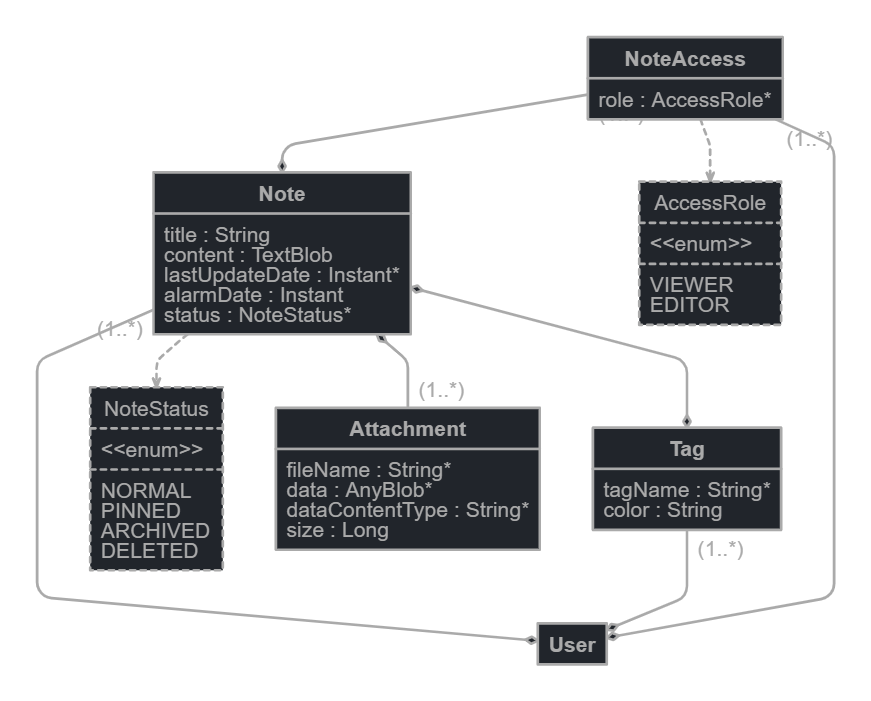
\includegraphics[width=\textwidth]{jhipster-jdl.png}
	\caption{Schema concettuale del dominio e relazione molti-a-molti tra note e tag.}
	\label{fig:er-dominio}
\end{figure}

\subsection{Gestione degli utenti e proprietà dei dati}
\label{subsec:proprieta-dati}

L’applicazione sfrutta il sistema di autenticazione integrato in JHipster per associare note e tag ai rispettivi utenti proprietari. Questo consente di garantire l’isolamento dei dati tra utenti differenti e di introdurre controlli di accesso negli endpoint REST, evitando che un utente possa leggere o modificare risorse non di sua proprietà.

\section{Test-Driven Development nel caso di studio}
\label{sec:tdd}
Questa sezione analizza l’applicazione del Test-Driven Development (TDD) all’interno del caso di studio sviluppato con JHipster. L’analisi viene condotta attraverso l’introduzione di test aggiuntivi relativi a vincoli di dominio non coperti dal semplice scaffolding CRUD.

Il TDD prevede che la scrittura del test preceda l’implementazione della funzionalità \cite{Beck2002,BettiniTDD}. In un progetto generato con JHipster, tuttavia, una parte significativa del codice applicativo e una suite iniziale di test vengono prodotti automaticamente. Ciò non rende impossibile l’adozione del TDD fin da subito: il TDD viene applicato in modo \emph{incrementale} sulle funzionalità aggiuntive o sui vincoli che emergono durante l’evoluzione del progetto.

\subsection{Analisi dei test generati automaticamente da JHipster}
\label{subsec:test-generati}

JHipster genera automaticamente una suite di test backend che copre principalmente le funzionalità CRUD e la correttezza degli endpoint REST. In particolare, per ciascuna entità vengono tipicamente prodotti test di integrazione basati su Spring Boot Test e MockMvc, che verificano l’accesso alle API, la serializzazione JSON, i codici di risposta HTTP e alcune validazioni di base.

Questi test risultano utili perché forniscono una base iniziale che intercetta rapidamente errori di configurazione, verifica che l’applicazione sia avviabile e funzionante, costituisce un primo strato di regressione automatica.

Tuttavia, tali test non derivano direttamente da requisiti di dominio espliciti, ma verificano prevalentemente la correttezza strutturale dell’applicazione (ad esempio: ``l’endpoint di creazione restituisce 201'', ``il campo obbligatorio non può essere nullo''). Inoltre, non coprono regole di business specifiche, che devono essere introdotte e testate manualmente.

\begin{figure}[H]
\dirtree{%
	.1 src/test/java/com/giovannip/noticeme/.
	.2 domain/.
	.3 AttachmentTest.java.
	.3 NoteTest.java.
	.3 TagTest.java.
	.2 service/.
	.3 dto/.
	.4 AttachmentDTOTest.java.
	.4 NoteDTOTest.java.
	.4 TagDTOTest.java.
	.3 mapper/.
	.4 AttachmentMapperTest.java.
	.4 NoteMapperTest.java.
	.4 TagMapperTest.java.
	.2 web/.
	.3 rest/.
	.4 AttachmentResourceIT.java.
	.4 NoteResourceIT.java.
	.4 TagResourceIT.java.
	.1 src/test/javascript/.
	.2 jest/ (example).
	.3 attachment.component.spec.ts.
	.3 note.component.spec.ts.
	.3 tag.component.spec.ts.
	.2 cypress/.
	.3 e2e/.
	.4 entity/.
	.5 attachment.cy.ts.
	.5 note.cy.ts.
	.5 note-access.cy.ts.
	.5 tag.cy.ts.
}
\caption{Estratto dell’albero dei test generati automaticamente}
\label{fig:test-tree}
\end{figure}

JHipster genera automaticamente una suite di test che copre sia il backend che il frontend dell'applicazione. In particolare, sono presenti test di integrazione per le API REST, test unitari per dominio, DTO e mapper, test unitari frontend tramite Jest e test end-to-end realizzati con Cypress.

\subsubsection{Test di integrazione con Spring Boot}
\label{sec:integration-test}

Oltre ai test unitari, l'applicazione utilizza test di integrazione per verificare il comportamento del sistema con il contesto applicativo completo, includendo controller REST, service layer, repository e configurazione di sicurezza.

Nel progetto sviluppato con JHipster, i test di integrazione sono organizzati principalmente nelle classi \texttt{*ResourceIT}, generate automaticamente per verificare gli endpoint REST.

\subsection{Applicazione del ciclo Red--Green--Refactor su un vincolo di dominio}
\label{subsec:red-green-refactor}

Per applicare il TDD, consideriamo un vincolo di business non garantito automaticamente dallo scaffolding delle entità: \emph{un utente può associare a una nota esclusivamente tag di sua proprietà}. È quindi necessario introdurre una logica applicativa nel service layer (o in uno strato equivalente) che verifichi la proprietà dei tag prima di effettuare l’associazione.

\subsubsection{Fase Red: definizione del comportamento atteso}
\label{subsec:red}

Nella fase iniziale è stato scritto un test di integrazione che formalizza il comportamento desiderato: dato un utente autenticato, proprietario della nota, l'aggiornamento deve fallire se tra i tag associati compare almeno un tag appartenente a un altro utente.

\Needspace{12\baselineskip}
\captionsetup{type=listing}
\captionof{listing}{Test TDD: rifiuto dell'associazione di un tag appartenente a un altro utente}
\label{lst:tdd-red-note-foreign-tag}
\begin{minted}[fontsize=\small,breaklines,autogobble]{java}
@Test
@Transactional
void putNoteShouldRejectTagOwnedByAnotherUser() throws Exception {
	User owner = getOrCreateUser(em, "user");
	User other = getOrCreateUser(em, "other");
	
	insertedNote = noteRepository.saveAndFlush(
		new Note()
			.title(DEFAULT_TITLE)
			.content(DEFAULT_CONTENT)
			.status(DEFAULT_STATUS)
			.owner(owner)
	);
	
	Tag foreignTag = new Tag()
		.tagName("foreign")
		.color("red")
		.owner(other);
	em.persist(foreignTag);
	em.flush();
	
	NoteDTO noteDTO = noteMapper.toDto(insertedNote);
	
	TagDTO foreignTagDTO = new TagDTO();
	foreignTagDTO.setId(foreignTag.getId());
	foreignTagDTO.setTagName(foreignTag.getTagName());
	foreignTagDTO.setColor(foreignTag.getColor());
	
	noteDTO.setTags(Set.of(foreignTagDTO));
	
	restNoteMockMvc
		.perform(
			put(ENTITY_API_URL_ID, insertedNote.getId())
				.contentType(MediaType.APPLICATION_JSON)
				.content(om.writeValueAsBytes(noteDTO))
		)
		.andExpect(status().isBadRequest());
	
	em.clear();
	Note persisted = noteRepository.findById(insertedNote.getId()).orElseThrow();
	assertThat(persisted.getTags()).isEmpty();
}
\end{minted}

L'operazione di aggiornamento della nota con il tag ``estraneo'' viene eseguita tramite un endpoint REST e il comportamento atteso è il rifiuto della richiesta con codice HTTP \texttt{400}.

\subsubsection{Fase Green: implementazione minima nel service layer}
\label{subsec:green}

Per evitare di caricare inutilmente tutte le entità \texttt{Tag}, è stata aggiunta nella repository una query derivata che conta quanti tag, tra quelli passati in input, appartengono all'utente corrente.

\Needspace{12\baselineskip}
\captionsetup{type=listing}
\captionof{listing}{Metodo di supporto aggiunto alla repository}
\label{lst:tdd-green-repository}
\begin{minted}{java}
	public interface TagRepository extends JpaRepository<Tag, Long> {
		
		long countByIdInAndOwnerLogin(Collection<Long> ids, String login);
		
	}
\end{minted}

Nel service layer, il controllo può essere implementato come segue:

\Needspace{12\baselineskip}
\captionsetup{type=listing}
\captionof{listing}{Implementazione minima del controllo nel service layer}
\label{lst:tdd-green-service}
\begin{minted}{java}
	@Service
	@Transactional
	public class NoteService {
		
		private final NoteRepository noteRepository;
		private final UserService userService;
		private final NoteMapper noteMapper;
		private final TagRepository tagRepository;
		
		public NoteService(
		NoteRepository noteRepository,
		NoteMapper noteMapper,
		UserService userService,
		TagRepository tagRepository
		) {
			this.noteRepository = noteRepository;
			this.userService = userService;
			this.noteMapper = noteMapper;
			this.tagRepository = tagRepository;
		}
		
		public NoteDTO update(NoteDTO noteDTO) {
			validateOwnedTags(noteDTO);
			
			Note existingNote = noteRepository
				.findById(noteDTO.getId())
				.orElseThrow(() -> new IllegalArgumentException(
					"Note not found with id " + noteDTO.getId()
				));
			
			noteMapper.partialUpdate(existingNote, noteDTO);
			existingNote = noteRepository.save(existingNote);
			return noteMapper.toDto(existingNote);
		}
		
		private void validateOwnedTags(NoteDTO noteDTO) {
			if (noteDTO.getTags() == null || noteDTO.getTags().isEmpty()) {
				return;
			}
			
			String currentLogin = SecurityUtils.getCurrentUserLogin()
				.orElseThrow(() -> new IllegalStateException("Current user not found"));
			
			Set<Long> tagIds = noteDTO.getTags().stream()
				.map(TagDTO::getId)
				.filter(Objects::nonNull)
				.collect(Collectors.toSet());
			
			if (tagIds.size() != noteDTO.getTags().size()) {
				throw new BadRequestAlertException(
					"Invalid tag list",
					"note",
					"taginvalid"
				);
			}
			
			long ownedTagCount = tagRepository.countByIdInAndOwnerLogin(tagIds, currentLogin);
			
			if (ownedTagCount != tagIds.size()) {
				throw new BadRequestAlertException(
					"A note can only use tags owned by the current user",
					"note",
					"foreigntag"
				);
			}
		}
	}
\end{minted}

L'utente autenticato viene recuperato tramite \texttt{SecurityUtils.getCurrentUserLogin()}, una utility per ottenere il login associato al contesto di sicurezza corrente. In questo modo la regola di dominio resta centralizzata nel service layer e non dipende dal client.

\subsubsection{Fase Refactor: consolidamento e pulizia}
\label{subsec:refactor}

Una volta superato il test, il codice è stato rifinito separando chiaramente la logica di validazione dal resto del flusso di aggiornamento \cite{Fowler2018}. In particolare, il controllo è stato estratto nel metodo privato \texttt{validateOwnedTags(...)}, con il vantaggio di ridurre la duplicazione: lo stesso controllo può essere richiamato non solo in \texttt{update(...)}, ma anche in \texttt{save(...)} e in \texttt{partialUpdate(...)}.

\subsection{Testing della relazione molti-a-molti Note--Tag}
\label{sec:test-moltimolti}

La relazione molti-a-molti tra \texttt{Note} e \texttt{Tag} rappresenta un punto sensibile nei test di integrazione, poiché coinvolge la join table generata automaticamente da JPA/Hibernate, la gestione delle collezioni e la serializzazione degli oggetti tramite endpoint REST.

Dal punto di vista del testing, è importante verificare che:

\begin{itemize}
	\item l'associazione tra note e tag venga salvata correttamente nella join table;
	\item uno stesso tag possa essere associato a più note;
	\item la rimozione di un tag da una nota aggiorni correttamente la relazione;
	\item la serializzazione JSON delle collezioni funzioni correttamente negli endpoint REST.
\end{itemize}

Il Listing~\ref{lst:note-tag-association-test} mostra un esempio di test di integrazione che verifica l'associazione di più tag a una singola nota.

\Needspace{12\baselineskip}
\captionsetup{type=listing}
\captionof{listing}{Test di integrazione della relazione Note--Tag}
\label{lst:note-tag-association-test}
\begin{minted}{java}
@Test
@Transactional
void shouldAssociateMultipleTagsToNote() throws Exception {
	User user = getOrCreateUser(em, "user");
	
	insertedNote =
	noteRepository.saveAndFlush(
		new Note()
			.title("Test note")
			.content("content")
			.status(NoteStatus.NORMAL)
			.owner(user)
	);
	
	Tag tag1 = tagRepository.saveAndFlush(
		new Tag().tagName("tag1").color("blue").owner(user)
	);
	
	Tag tag2 = tagRepository.saveAndFlush(
		new Tag().tagName("tag2").color("red").owner(user)
	);
	
	NoteDTO dto = noteMapper.toDto(insertedNote);
	
	TagDTO t1 = new TagDTO();
	t1.setId(tag1.getId());
	
	TagDTO t2 = new TagDTO();
	t2.setId(tag2.getId());
	
	dto.setTags(Set.of(t1, t2));
	
	restNoteMockMvc.perform(
		put(ENTITY_API_URL_ID, insertedNote.getId())
			.contentType(MediaType.APPLICATION_JSON)
			.content(om.writeValueAsBytes(dto))
	).andExpect(status().isOk());
	
	em.clear();
	
	Note persisted = noteRepository.findById(insertedNote.getId()).orElseThrow();
	
	assertThat(persisted.getTags()).hasSize(2);
}
\end{minted}

Il test crea una nota e due tag appartenenti allo stesso utente, invia una richiesta REST di aggiornamento della nota e verifica successivamente, interrogando il database, che la collezione dei tag associati contenga effettivamente due elementi. In questo modo si verifica implicitamente anche la corretta persistenza della join table generata da JPA.

\section{Unit testing frontend con Jest}
\label{sec:jest}

Per il testing del frontend Angular è stato utilizzato \texttt{Jest}, framework di unit testing integrato nel progetto generato da JHipster. Jest consente di verificare in modo rapido e isolato il comportamento di componenti, servizi e classi di supporto del frontend, senza richiedere l’avvio completo dell’applicazione o l’interazione con un browser reale.

L’attenzione si concentra quindi sulla logica lato client, sulla gestione dello stato del componente e sulla corretta interazione con i servizi Angular. Nel progetto i test Jest sono collocati accanto ai file del frontend. Per l’entità \texttt{Note}, ad esempio, JHipster ha generato automaticamente test per:
\begin{itemize}
	\item il componente di lista \texttt{note.component.spec.ts};
	\item il servizio REST \texttt{note.service.spec.ts};
	\item il servizio di gestione del form \texttt{note-form.service.spec.ts};
	\item il componente di aggiornamento \texttt{note-update-dialog.component.spec.ts}.
\end{itemize}

\subsection{Esempi di test generati}
\label{subsec:jest-esempi}

JHipster genera verifiche per le principali operazioni CRUD lato client: ricerca di un elemento, creazione, aggiornamento completo, aggiornamento parziale, recupero della lista ed eliminazione. I test utilizzano \texttt{HttpTestingController} per simulare le richieste HTTP e verificare che il service costruisca correttamente le chiamate REST e trasformi i dati restituiti dal backend nel modello TypeScript usato dal frontend.

\Needspace{12\baselineskip}
\captionsetup{type=listing}
\captionof{listing}{Estratto semplificato di test Jest per il service delle note}
\label{lst:jest-note-service}
\begin{minted}[linenos]{typescript}
	describe('Note Service', () => {
		let service: NoteService;
		let httpMock: HttpTestingController;
		let expectedResult: INote | INote[] | boolean | null;
		
		beforeEach(() => {
			TestBed.configureTestingModule({
				providers: [provideHttpClient(), provideHttpClientTesting()],
			});
			service = TestBed.inject(NoteService);
			httpMock = TestBed.inject(HttpTestingController);
		});
		
		it('should find an element', () => {
			service.find(123).subscribe(resp => (expectedResult = resp.body));
			
			const req = httpMock.expectOne({ method: 'GET' });
			req.flush(returnedFromService);
			
			expect(expectedResult).toMatchObject(expected);
		});
		
		it('should delete a Note', () => {
			service.delete(123).subscribe(resp => (expectedResult = resp.ok));
			
			const req = httpMock.expectOne({ method: 'DELETE' });
			req.flush({ status: 200 });
			
			expect(expectedResult).toBe(true);
		});
	});
\end{minted}

\section{Behavior-Driven Development con Cucumber}
\label{sec:bdd-cucumber}

Per formalizzare comportamenti ad alto livello è possibile integrare Cucumber, framework che consente di descrivere scenari di utilizzo attraverso il linguaggio Gherkin. Questo approccio permette di esprimere i requisiti funzionali in una forma leggibile anche da soggetti non tecnici, favorendo la comunicazione tra sviluppatori e stakeholder.

Un esempio di scenario sviluppato nel caso di studio è riportato nel Listing~\ref{lst:gherkin-scenario}.

\Needspace{12\baselineskip}
\captionsetup{type=listing}
\captionof{listing}{Esempio di scenario Gherkin}
\label{lst:gherkin-scenario}
\begin{minted}{gherkin}
	Feature: Gestione delle note
	
	Scenario: Creazione di una nota con due tag
	Given l'utente autenticato ha creato i tag "Studio" e "Lavoro"
	When crea una nota con titolo "Preparare esame"
	And associa i tag "Studio" e "Lavoro"
	Then la nota deve essere salvata con 2 tag associati
\end{minted}

Gli scenari Gherkin vengono poi collegati al codice applicativo tramite le \textit{step definitions}, implementate in Java e integrate con il contesto Spring Boot. Ogni passo descritto nello scenario viene associato a un metodo che esegue le operazioni necessarie e verifica gli effetti prodotti sul sistema. Le step definitions possono interagire con i service applicativi oppure con gli endpoint REST, a seconda del livello di astrazione scelto per il test.

\Needspace{12\baselineskip}
\captionsetup{type=listing}
\captionof{listing}{Esempio semplificato di step definition}
\label{lst:cucumber-step}
\begin{minted}{java}
	@WithMockUser(username = "user")
	public class GestioneNoteStepDefs extends StepDefs {
		
		@Autowired
		private EntityManager em;
		
		@Autowired
		private TagRepository tagRepository;
		
		@Autowired
		private NoteRepository noteRepository;
		
		private Note notaCreata;
		private final Set<Tag> tagDaAssociare = new HashSet<>();
		
		@Before
		public void cleanScenarioState() {
			notaCreata = null;
			tagDaAssociare.clear();
		}
		
		@Given("l'utente autenticato ha creato i tag {string} e {string}")
		public void utenteHaCreatoITag(String nomeTag1, String nomeTag2) {
			Tag tag1 = creaTagSeAssente(nomeTag1);
			Tag tag2 = creaTagSeAssente(nomeTag2);
			
			tagDaAssociare.add(tag1);
			tagDaAssociare.add(tag2);
		}
		
		@When("crea una nota con titolo {string}")
		public void creaUnaNotaConTitolo(String titolo) {
			User owner = getOrCreateUser("user");
			
			Note note = new Note()
				.title(titolo)
				.content("contenuto di test")
				.status(NoteStatus.NORMAL)
				.owner(owner);
			
			notaCreata = noteRepository.saveAndFlush(note);
		}
	}
\end{minted}

JHipster, tuttavia, non genera molto oltre la configurazione base di Cucumber. Nel caso in esame, il framework si limita essenzialmente a fornire uno scenario di esempio, riportato nel Listing~\ref{lst:gherkin-scenario-gen}.

\Needspace{12\baselineskip}
\captionsetup{type=listing}
\captionof{listing}{Scenario generato}
\label{lst:gherkin-scenario-gen}
\begin{minted}{gherkin}
	Feature: User management
	
	Scenario: Retrieve administrator user
	When I search user 'admin'
	Then the user is found
	And his last name is 'Administrator'
\end{minted}

\begin{figure}[H]
	\centering
	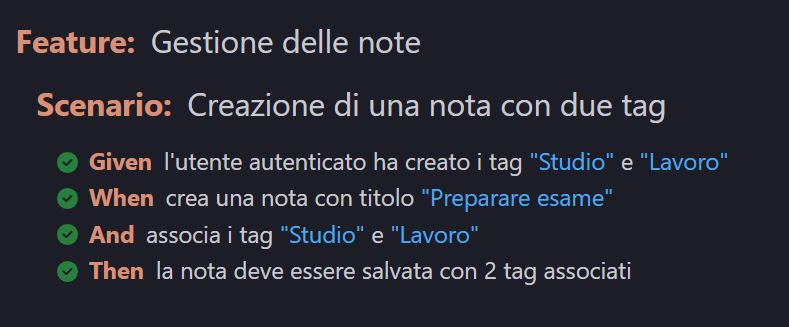
\includegraphics[width=\textwidth]{cucumber.png}
	\caption{Report di Cucumber.}
	\label{fig:cucumber-reports}
\end{figure}

\section{End-to-End Testing con Cypress}
\label{sec:cypress}

Per testare l'applicazione dal punto di vista dell'utente finale viene integrato Cypress, uno strumento dedicato ai test end-to-end per applicazioni web. Cypress consente di eseguire il browser in modalità controllata e simulare interazioni reali con l'interfaccia Angular, verificando non solo la correttezza delle singole chiamate HTTP, ma soprattutto il comportamento complessivo dell'applicazione durante l'interazione utente \cite{CypressDocs}.

I test Cypress generati dal progetto coprono già diversi aspetti dell’applicazione, in particolare:

\begin{itemize}
	\item autenticazione dell’utente;
	\item navigazione tra le pagine;
	\item accesso alle pagine CRUD delle entità;
\end{itemize}

I test generati automaticamente mostrano già la struttura generale degli scenari end-to-end: apertura della pagina dell’entità, accesso al form di creazione, visualizzazione della pagina di dettaglio, modifica e ritorno alla lista.

Tuttavia, nel caso di studio considerato, l'interfaccia relativa alle note è stata personalizzata rispetto al CRUD standard generato da JHipster. Per questo motivo i test pregenerati relativi all'entità \texttt{Note} non risultano aderenti al comportamento reale della UI e sono stati quindi adattati.

In particolare, sono stati implementati questi test specifici per verificare tre scenari applicativi:

\begin{itemize}
	\item creazione di una nuova nota e verifica della sua comparsa nella lista;
	\item creazione di una nota con associazione immediata di un tag;
	\item apertura del dialog di modifica di una nota esistente e aggiunta di un ulteriore tag, con verifica dell'aggiornamento nell'interfaccia.
\end{itemize}

Il Listing~\ref{lst:cypress-test} mostra un estratto di un test Cypress. Lo scenario esegue l'accesso alla pagina delle note, crea una nuova nota, apre il dialog di aggiornamento tramite selezione della card corrispondente e aggiunge un nuovo tag, verificando sia la corretta risposta HTTP sia l'effettiva presenza dei tag nella lista delle note.

\Needspace{12\baselineskip}
\captionsetup{type=listing}
\captionof{listing}{Test end-to-end con Cypress per creazione e aggiornamento di una nota}
\label{lst:cypress-test}
\begin{minted}[linenos]{typescript}
it('should create a note, open update dialog, add a tag and show both in UI', () => {
	const title = `E2E dialog tag note ${Date.now()}`;
	const content = 'Nota da aggiornare dal dialog';
	const initialTag = `iniziale-${Date.now()}`;
	const addedTag = `aggiunto-${Date.now()}`;
	
	cy.visit('/note');
	cy.wait('@getNotes');
	
	cy.get('[data-cy="title"]').clear().type(title);
	cy.get('[data-cy="content"]').clear().type(content);
	cy.get('[data-cy="tagInput"]').first().type(`${initialTag}{enter}`);
	cy.get('[data-cy="NoteSaveButton"]').click();
	
	cy.wait('@postNote').then(({ response }) => {
		expect(response?.statusCode).to.eq(201);
	});
	
	cy.contains('[data-cy="noteTitle"]', title).should('be.visible');
	
	cy.contains('[data-cy="noteCard"] [data-cy="noteTitle"]', title)
		.closest('[data-cy="noteCard"]')
		.click();
	
	cy.get('[data-cy="noteUpdateDialog"]')
		.should('be.visible')
		.within(() => {
			cy.contains('[data-cy="tagChip"]', initialTag).should('be.visible');
			cy.get('[data-cy="tagInput"]').type(`${addedTag}{enter}`);
			cy.get('[data-cy="NoteSaveEdit"]').click({ force: true });
		});
	
	cy.wait('@patchNote').then(({ response }) => {
		expect(response?.statusCode).to.eq(200);
	});
	
	cy.contains('[data-cy="noteCard"] [data-cy="noteTitle"]', title)
		.closest('[data-cy="noteCard"]')
		.within(() => {
			cy.contains('[data-cy="tagChip"]', initialTag).should('be.visible');
			cy.contains('[data-cy="tagChip"]', addedTag).should('be.visible');
		});
});
\end{minted}

I test Cypress possono essere eseguiti sia in ambiente di sviluppo sia in modalità automatizzata. Durante lo sviluppo conviene utilizzare l'interfaccia grafica di Cypress, che consente di osservare passo per passo i comandi eseguiti, il DOM renderizzato e le chiamate HTTP intercettate. In fase di esecuzione automatizzata, invece, la suite può essere avviata in modalità \emph{headless}, modalità adatta alle pipeline CI.

\section{Mutation Testing con PIT}
\label{sec:pit}

Per valutare non solo la copertura del codice ma anche l'effettiva capacità dei test di individuare errori nel comportamento del sistema, è possibile introdurre il \textit{mutation testing} tramite lo strumento PIT (\textit{Pitest}). 

A differenza della semplice copertura del codice, il mutation testing introduce modifiche artificiali nel codice sorgente, chiamate \textit{mutanti}, per verificare se i test sono in grado di individuare tali variazioni. Se un mutante viene rilevato da almeno un test, esso viene considerato ``ucciso''; in caso contrario, indica una possibile debolezza nella suite di test \cite{BettiniTDD,PITDocs}.

Per integrare PIT con JHipster è sufficiente aggiungere il plugin Maven nel file \texttt{pom.xml}, come mostrato nel Listing~\ref{lst:pit-plugin}.

\Needspace{12\baselineskip}
\captionsetup{type=listing}
\captionof{listing}{Configurazione Maven del plugin PIT}
\label{lst:pit-plugin}
\begin{minted}{xml}
<plugin>
	<groupId>org.pitest</groupId>
	<artifactId>pitest-maven</artifactId>
	<version>${pitest.version}</version>
	<dependencies>
		<dependency>
			<groupId>org.pitest</groupId>
			<artifactId>pitest-junit5-plugin</artifactId>
			<version>${pitest-junit5.version}</version>
		</dependency>
	</dependencies>
	<configuration>
		<targetClasses>
			<param>com.giovannip.*</param>
		</targetClasses>
		<targetTests>
			<param>com.giovannip.*</param>
		</targetTests>
		<excludedClasses>
			<param>com.giovannip.noticeme.service.mapper.*MapperImpl</param>
		</excludedClasses>
		<excludedTestClasses>
			<param>com.giovannip.noticeme.TechnicalStructureTest</param>
			<param>com.giovannip.noticeme.*Architecture*</param>
			<param>com.giovannip.noticeme.*ArchUnit*</param>
			<param>com.giovannip.noticeme.*Structure*</param>
			<param>com.giovannip.noticeme.cucumber.*</param>
			<param>gatling.simulations.*</param>
		</excludedTestClasses>
		<mutationThreshold>1</mutationThreshold>
		<avoidCallsTo>
			<param>java.util.logging</param>
			<param>org.slf4j</param>
		</avoidCallsTo>
		<threads>4</threads>
		<outputFormats>
			<param>HTML</param>
		</outputFormats>
	</configuration>
</plugin>
\end{minted}

L'esecuzione dell'analisi avviene tramite il comando seguente; naturalmente, PIT è in grado di produrre un risultato significativo solo se la suite di test viene eseguita senza errori:

\Needspace{12\baselineskip}
\begin{minted}{bash}
	./mvnw org.pitest:pitest-maven:mutationCoverage
\end{minted}

Al termine dell'esecuzione, PIT genera automaticamente un report HTML contenente statistiche dettagliate sul numero di mutanti generati, sul numero di mutanti uccisi dai test e sui mutanti sopravvissuti. Il report permette inoltre di analizzare a livello di singola classe quali mutazioni non vengono rilevate dalla suite di test.

La Figura~\ref{fig:pit-overview} mostra un esempio della schermata principale del report generato da PIT.

\begin{figure}[H]
	\centering
	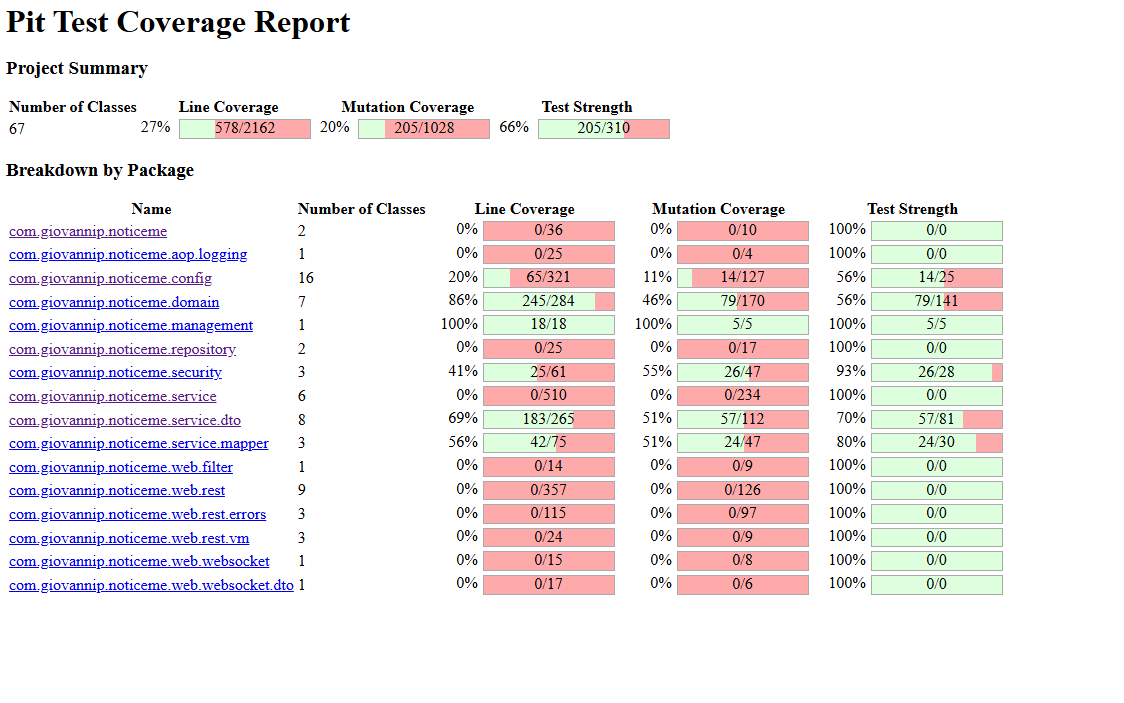
\includegraphics[width=0.9\textwidth]{pit-overview.png}
	\caption{Panoramica del report generato da Pitest.}
	\label{fig:pit-overview}
\end{figure}

I risultati ottenuti nel caso di studio mostrano che, nonostante una buona copertura strutturale del codice evidenziata dai report JaCoCo, una parte significativa dei mutanti sopravvive all'esecuzione dei test. Questo risultato è coerente con la natura della suite di test del progetto, composta in larga misura da test di integrazione orientati alla verifica del comportamento dell'applicazione tramite API REST. Sebbene tali test coprano ampie porzioni di codice, nella configurazione generata da JHipster essi non contribuiscono in modo efficace all'analisi di mutation testing condotta da PIT, che in questo contesto si focalizza sui soli test unitari.

\section{Performance Testing con Gatling}
\label{sec:gatling}

JHipster può integrare automaticamente Gatling come strumento per l'esecuzione di test di performance sulle API REST. Gatling consente di simulare un numero elevato di utenti concorrenti e di raccogliere metriche quali tempo medio di risposta, throughput e percentili di latenza \cite{GatlingDocs}.

Nel progetto generato, Gatling è integrato tramite dipendenze Maven e tramite il plugin \texttt{gatling-maven-plugin}, che consente di eseguire le simulazioni direttamente durante la fase di testing del progetto.

Le simulazioni Gatling generate automaticamente da JHipster si trovano nel package \texttt{gatling.simulations}. Per ogni entità REST esposta dall'applicazione viene creata una simulazione che verifica il comportamento delle principali operazioni CRUD sotto carico.

\subsection{Struttura dei test pregenerati}
La simulazione \texttt{NoteGatlingTest} esegue una sequenza di richieste HTTP che riproduce un utilizzo realistico dell'API dell'applicazione.

Lo scenario segue la sequenza:

\begin{itemize}
	\item tentativo di accesso senza autenticazione;
	\item autenticazione tramite endpoint \texttt{/api/authenticate};
	\item verifica dell'accesso autenticato all'endpoint \texttt{/api/account};
	\item esecuzione delle principali operazioni CRUD sull'entità \texttt{Note}.
\end{itemize}

Il Listing~\ref{lst:gatling-scenario} mostra un estratto semplificato dello scenario principale della simulazione.

\Needspace{12\baselineskip}
\captionsetup{type=listing}
\captionof{listing}{Estratto semplificato della simulazione Gatling per l'entità Note}
\label{lst:gatling-scenario}
\begin{minted}{java}
	ChainBuilder scn =
		exec(http("First unauthenticated request")
			.get("/api/account")
			.check(status().is(401)))
			
			.exec(http("Authentication")
			.post("/api/authenticate")
			.body(StringBody("{\"username\":\"admin\",\"password\":\"admin\"}"))
			.check(header("Authorization").saveAs("access_token")))
			
			.exec(http("Authenticated request")
			.get("/api/account")
			.check(status().is(200)))
			
			.exec(http("Get all notes")
			.get("/api/notes"))
			
			.exec(http("Create new note")
			.post("/api/notes"));
			
			.exec(http("Get created note")
			.get("#{new_note_url}")
			
			.exec(http("Delete created note")
			.delete("#{new_note_url}")
\end{minted}

Questo scenario consente di verificare non solo la correttezza delle risposte HTTP, ma anche il comportamento delle API in presenza di richieste concorrenti.

\subsection{Simulazione del carico}
Il carico viene introdotto tramite la strategia \texttt{rampUsers}, che simula un aumento progressivo degli utenti virtuali.

\Needspace{12\baselineskip}
\captionsetup{type=listing}
\captionof{listing}{Configurazione dell'iniezione di utenti virtuali}
\begin{minted}{java}
	setUp(
		users.injectOpen(
			rampUsers(Integer.getInteger("users", 100))
				.during(Duration.ofMinutes(Integer.getInteger("ramp", 1)))
		)
	);
\end{minted}

Nella configurazione predefinita, Gatling simula 100 utenti virtuali distribuiti nell'arco di 1 minuto. Questo approccio consente di osservare come il sistema reagisce all'aumento progressivo del carico, evitando picchi improvvisi di richieste. I parametri possono essere modificati durante l'esecuzione del test, permettendo di adattare facilmente il carico simulato. Per eseguire i test Gatling è necessario che l'applicazione sia già in esecuzione su una porta raggiungibile; per questo motivo tali test risultano particolarmente adatti a essere eseguiti in ambienti di staging o di integrazione continua, piuttosto che durante lo sviluppo locale.

\Needspace{12\baselineskip}
\begin{minted}{shell}
	./mvnw gatling:test -Dusers=200 -Dramp=2
\end{minted}

Al termine dell'esecuzione Gatling genera automaticamente un report HTML contenente le principali metriche di performance, come mostrato nella Figura~\ref{fig:gatling-report}.

\begin{figure}[H]
	\centering
	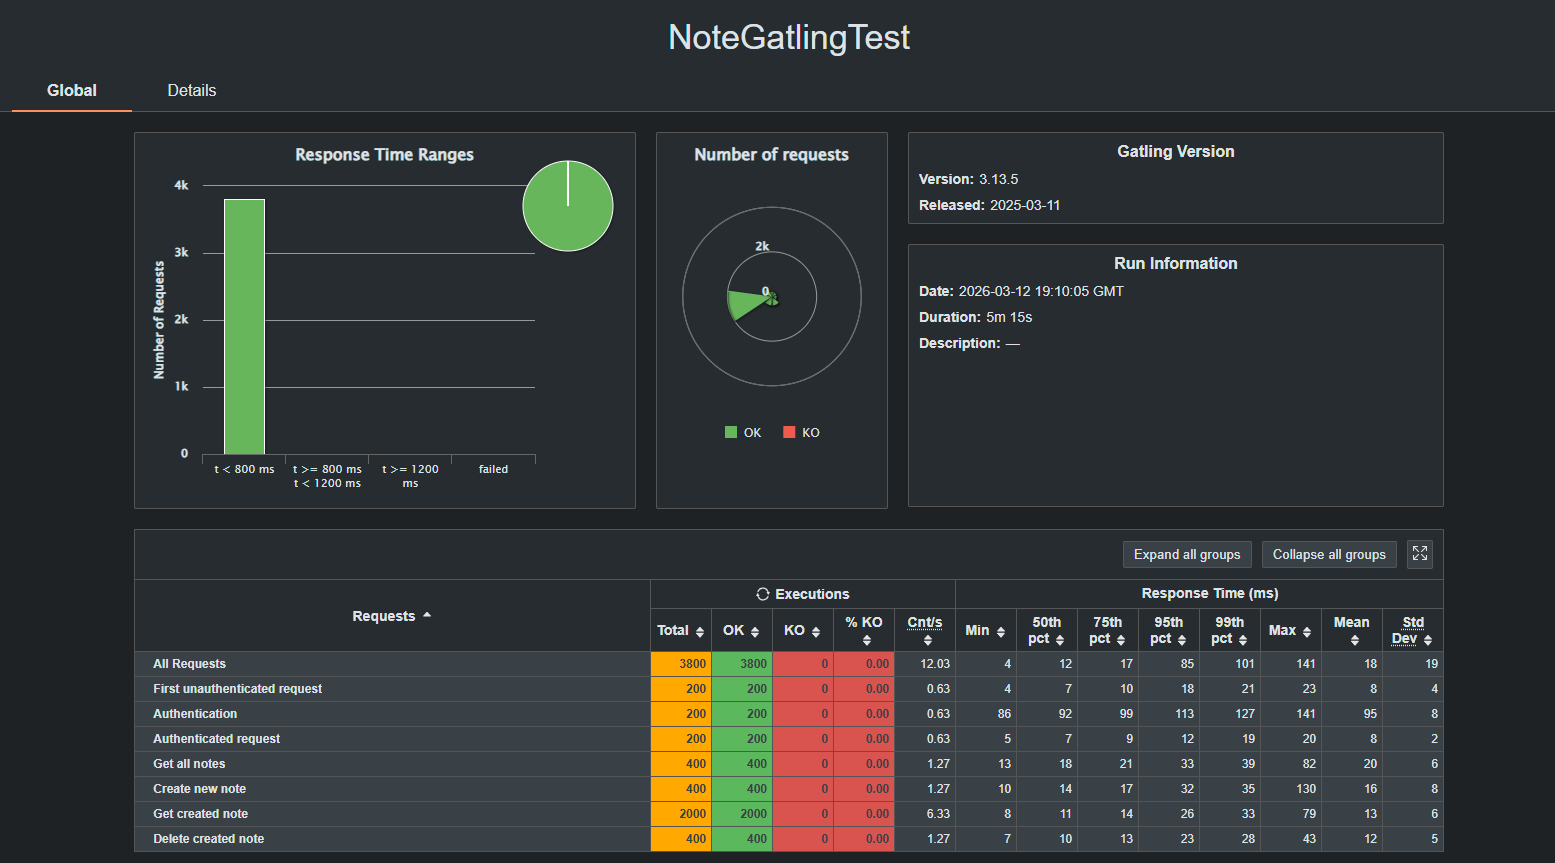
\includegraphics[width=\textwidth]{gatling-overview.png}
	\caption{Panoramica del report di performance generato da Gatling al termine della simulazione.}
	\label{fig:gatling-report}
\end{figure}

\subsection{Analisi dei report di performance}

I report generati da Gatling includono informazioni quali:

\begin{itemize}
	\item numero totale di richieste
	\item percentuale di richieste riuscite e fallite
	\item tempo minimo, medio e massimo di risposta
	\item percentili di latenza (quanto velocemente risponde il sistema nella maggior parte dei casi)
	\item throughput nel tempo (numero di richieste gestite dal sistema per secondo)
\end{itemize}

\begin{figure}[H]
	\centering
	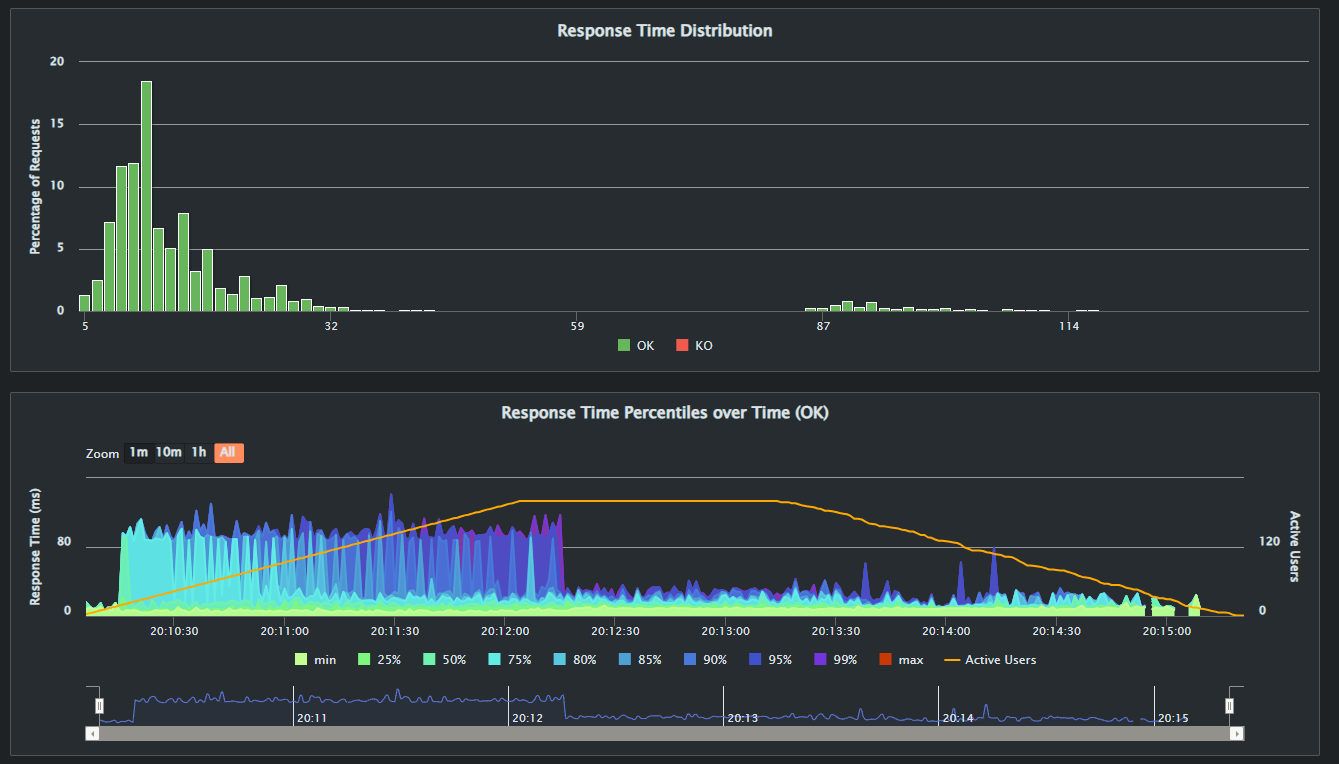
\includegraphics[width=0.9\textwidth]{gatling-response-time.png}
	\caption{Distribuzione dei tempi di risposta durante l'esecuzione del test di carico.}
	\label{fig:gatling-response}
\end{figure}


Questi grafici consentono di identificare eventuali colli di bottiglia nelle API e di valutare la scalabilità del sistema sotto carico.

\begin{figure}[H]
	\centering
	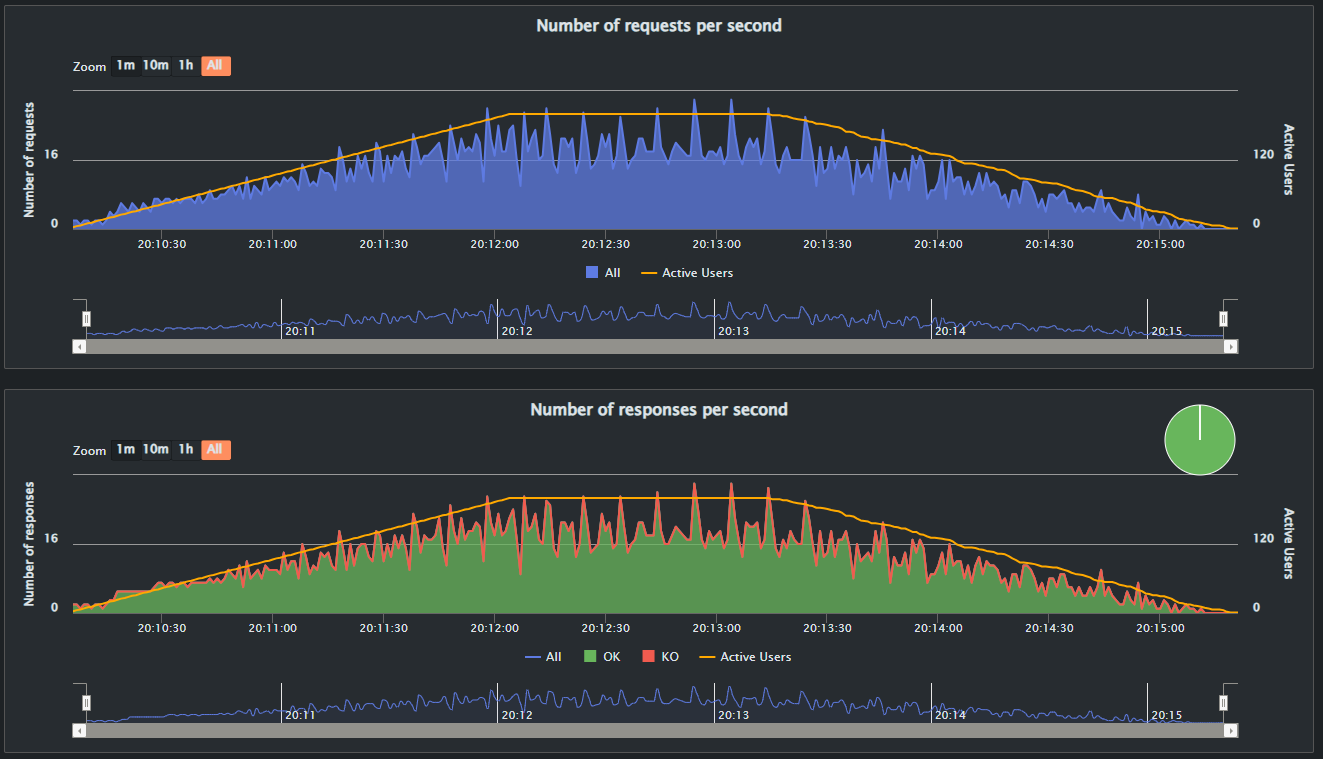
\includegraphics[width=0.9\textwidth]{gatling-throughput.png}
	\caption{Throughput del sistema espresso come numero di richieste al secondo durante la simulazione.}
	\label{fig:gatling-throughput}
\end{figure}

\subsection{Personalizzazione degli scenari di test}

I test generati automaticamente rappresentano una base iniziale per il performance testing. In contesti reali, tuttavia, è spesso necessario personalizzare gli scenari per riflettere in modo più accurato i comportamenti degli utenti.

Tra le principali estensioni possibili rientrano la simulazione di diversi profili di utenti (ad esempio anonimi, autenticati e amministratori), l’introduzione di sequenze di chiamate API che riproducano comportamenti differenti sull’applicazione e l’aumento progressivo del numero di utenti virtuali per valutare la scalabilità del sistema.

Gatling supporta inoltre strategie di iniezione più avanzate, come \texttt{constantUsersPerSec} o \texttt{stressPeakUsers}, che permettono di simulare scenari di carico più complessi.

\subsection{Ruolo del performance testing nel contesto della tesi}

Nel contesto della presente tesi i test di performance non costituiscono il focus principale dell'analisi, che è invece orientata alle pratiche di testing automatizzato e Continuous Integration.

Tuttavia, la presenza di Gatling all'interno dello stack JHipster dimostra come il framework favorisca un processo di verifica della qualità del software più ampio, includendo anche la validazione di requisiti non funzionali quali prestazioni e scalabilità.

\chapter{Integrazione continua nel caso di studio}
\label{cap:ci}

Questo capitolo descrive l’infrastruttura di Continuous Integration e le scelte effettuate per automatizzare build, test e analisi di qualità del progetto. La soluzione adottata consiste in un ambiente CI locale basato su Jenkins e Docker, integrato con SonarQube, un registry Docker locale e gli strumenti di test discussi nei capitoli precedenti.

JHipster mette a disposizione configurazioni pronte per pipeline CI attraverso il CLI (ad esempio per GitHub Actions, GitLab CI o Jenkins). Tuttavia, nel caso di studio tali configurazioni non risultavano pienamente compatibili con le esigenze del progetto; per questo motivo è stato realizzato un \texttt{Jenkinsfile} personalizzato, affiancato da un file \texttt{Docker Compose} per la creazione di una pipeline CI locale \cite{JHipsterDocs,JenkinsDocs,DockerDocs}.

\section{Infrastruttura CI locale basata su Docker}
\label{sec:infra-docker}

Per rendere l'ambiente facilmente riproducibile, i servizi necessari alla pipeline sono stati orchestrati tramite \texttt{Docker Compose}.

L'infrastruttura utilizzata nel caso di studio comprende i seguenti componenti principali:

\begin{itemize}
	\item Jenkins, responsabile dell'esecuzione della pipeline;
	\item SonarQube, utilizzato per l'analisi statica del codice e la valutazione dei quality gate;
	\item un database PostgreSQL dedicato al funzionamento di SonarQube;
	\item un registry Docker locale per la pubblicazione delle immagini generate.
\end{itemize}

Il Listing~\ref{lst:docker-compose-ci} mostra un estratto della configurazione \texttt{Docker Compose}. La configurazione completa è disponibile nel repository del progetto.

\Needspace{12\baselineskip}
\captionsetup{type=listing}
\captionof{listing}{Estratto del Docker Compose per l'ambiente CI locale}
\label{lst:docker-compose-ci}
\begin{minted}{yaml}
networks:
  ci-net:

services:
  sonar-db:
    image: postgres:16
    environment:
      POSTGRES_USER: sonar
      POSTGRES_PASSWORD: sonar
      POSTGRES_DB: sonar

  sonarqube:
    image: sonarqube:community
    depends_on:
      - sonar-db
    ports:
      - "19000:9000"

  registry:
    image: registry
    ports:
      - "15000:5000"

  jenkins:
    image: jenkins/jenkins:lts
    user: root
    ports:
      - "18080:8080"
      - "50000:50000"
    depends_on:
      - sonarqube
      - registry
\end{minted}

\section{Pipeline Jenkins: struttura e strategia multi-branch}
\label{sec:pipeline-jenkins}

La pipeline è stata implementata tramite un \texttt{Jenkinsfile} dichiarativo. La strategia adottata differenzia le attività in base al tipo di branch e al contesto di esecuzione:

\begin{itemize}
	\item sulle \emph{pull request} viene eseguita una suite rapida di unit test;
	\item sui branch \texttt{feature/*} viene eseguito un controllo qualità intermedio con raccolta di metriche;
	\item sul branch \texttt{dev} viene eseguita una suite completa, comprensiva di report Cucumber e, opzionalmente, di test più onerosi;
	\item sul branch \texttt{main} viene eseguita la build di rilascio e il packaging per la produzione.
\end{itemize}

Questa strategia consente, da un lato, di ottenere feedback rapido durante lo sviluppo e, dall’altro, di eseguire verifiche più approfondite prima dell’integrazione definitiva del codice.

\subsection{Validazione rapida su Pull Request}
Per le pull request la pipeline esegue una suite rapida di test, con l’obiettivo di fornire feedback immediato prima del merge.

\Needspace{12\baselineskip}
\captionsetup{type=listing}
\captionof{listing}{Estratto Jenkinsfile: validazione PR}
\label{lst:jenkins-pr}
\begin{minted}{groovy}
	stage('pr-validation') {
		when { changeRequest() }
		steps {
			sh './mvnw -ntp -Pdev,webapp,no-liquibase,frontend-test clean test'
		}
		post {
			always {
				junit allowEmptyResults: true, testResults: '**/target/surefire-reports/*.xml'
			}
		}
	}
\end{minted}

\subsection{Suite completa su branch \texttt{dev} e raccolta report}

Sul branch \texttt{dev} viene eseguita una suite più completa, comprensiva di test di integrazione e della generazione dei principali report. In questa fase vengono raccolti i report JUnit (\texttt{surefire}) e (\texttt{failsafe}), pubblicati i report di copertura tramite JaCoCo e, quando presenti, i report Cucumber.

\Needspace{12\baselineskip}
\captionsetup{type=listing}
\captionof{listing}{Estratto Jenkinsfile: suite completa su dev e report}
\label{lst:jenkins-dev}
\begin{minted}{groovy}
	stage('dev-full-qa') {
		when { branch 'dev' }
		steps {
			sh './mvnw -ntp -Pdev,webapp,frontend-test verify'
		}
		post {
			always {
				cucumber fileIncludePattern: '**/cucumber-reports/*.json'
				junit allowEmptyResults: true, testResults: '**/target/surefire-reports/*.xml'
				junit allowEmptyResults: true, testResults: '**/target/failsafe-reports/*.xml'
				publishHTML(target: [
				reportDir: 'target/site/jacoco',
				reportFiles: 'index.html',
				reportName: 'Jacoco Coverage'
				])
			}
		}
	}
\end{minted}

\subsection{Test ad alto costo computazionale}
\label{sub:heavy-tests}

Alcuni strumenti di verifica della qualità, come il Mutation Testing e i test di performance, richiedono tempi di esecuzione significativamente più lunghi rispetto ai test tradizionali. Per questo motivo tali verifiche vengono eseguite solo in condizioni specifiche.

Nel caso di studio, l'esecuzione dei test ad alto costo computazionale può essere attivata in due modi:

\begin{itemize}
	\item manualmente tramite il parametro della pipeline \texttt{RUN\_HEAVY};
	\item automaticamente se il messaggio di commit contiene tag specifici come \texttt{[heavy]} o \texttt{[perf]}.
\end{itemize}

\Needspace{12\baselineskip}
\captionsetup{type=listing}
\captionof{listing}{Estratto Jenkinsfile: PIT e Gatling condizionali}
\label{lst:jenkins-heavy}
\begin{minted}{groovy}
	stage('Heavy Tests (optional)') {
		when {
			allOf {
				branch 'dev'
				anyOf {
					expression { params.RUN_HEAVY }
					expression { env.COMMIT_MSG.contains('[heavy]') }
					expression { env.COMMIT_MSG.contains('[perf]') }
				}
			}
		}
		steps {
			sh './mvnw org.pitest:pitest-maven:mutationCoverage'
			sh './mvnw -ntp -Pdev,webapp -DskipTests package'
			sh '''
				nohup java -jar target/*.jar > app.log 2>&1 &
				echo $! > app.pid
			'''
			
			sh '''
				for i in $(seq 1 60); do
					if curl -fsS http://localhost:8080/management/health | grep -q '"status":"UP"'; then
						echo "Application is UP"
						exit 0
					fi
					sleep 5
				done
				echo "Application failed to start"
				tail -100 app.log || true
				exit 1
			'''  
			sh './mvnw gatling:test'
		}
		post {
			always {
				sh '''
					if [ -f app.pid ]; then
					kill $(cat app.pid) || true
					fi
				'''
				archiveArtifacts artifacts: 'target/pit-reports/**', fingerprint: true
				archiveArtifacts artifacts: 'target/gatling/**', fingerprint: true
			}
		}
	}
\end{minted}

\subsection{Analisi statica e Quality Gate con SonarQube}
\label{sub:sonar}

Per la valutazione automatica della qualità del codice è stato integrato SonarQube all'interno della pipeline Jenkins. L'analisi statica viene eseguita sul branch \texttt{dev} e utilizza i report di copertura generati da JaCoCo \cite{SonarQubeDocs}.

Al termine dell'analisi viene valutato il \textit{Quality Gate}, che rappresenta un insieme di criteri minimi di qualità (ad esempio copertura del codice, presenza di bug o code smells). Nel caso in cui il Quality Gate non venga superato, la pipeline viene interrotta.

\Needspace{12\baselineskip}
\captionsetup{type=listing}
\captionof{listing}{Estratto Jenkinsfile: analisi SonarQube}
\label{lst:jenkins-sonar-analysis}
\begin{minted}{groovy}
	stage('Sonar Analysis') {
		when { branch 'dev' }
		steps {
			withSonarQubeEnv('sonar') {
				script {
					def reports = 'target/site/jacoco/jacoco.xml'
					if (fileExists('target/pit-reports/jacoco.xml')) {
						reports += ',target/pit-reports/jacoco.xml'
					}
					sh """
					./mvnw sonar:sonar \
					-Dsonar.coverage.jacoco.xmlReportPaths=\${reports}
					"""
				}
			}
		}
	}
\end{minted}

\Needspace{12\baselineskip}
\captionsetup{type=listing}
\captionof{listing}{Estratto Jenkinsfile: verifica del Quality Gate}
\label{lst:jenkins-quality-gate}
\begin{minted}{groovy}
	stage('Quality Gate') {
		when { branch 'dev' }
		steps {
			timeout(time: 20, unit: 'MINUTES') {
				waitForQualityGate abortPipeline: true
			}
		}
	}
\end{minted}

Al termine dell’analisi, SonarQube mette a disposizione una dashboard che sintetizza lo stato qualitativo del progetto attraverso diverse metriche. Tra queste risultano particolarmente rilevanti l’esito del \textit{Quality Gate}, la copertura del codice e il numero di problemi individuati dall’analisi statica.

La Figura~\ref{fig:sonar-quality-gate} mostra la pagina principale del progetto su SonarQube, nella quale è possibile osservare immediatamente l’esito del \textit{Quality Gate}. La Figura~\ref{fig:sonar-overview-img} riporta invece la sezione \textit{Overview}, che raccoglie le principali metriche di qualità del progetto. Infine, la Figura~\ref{fig:sonar-issues} mostra la lista dei problemi individuati dall’analisi statica, tra cui \textit{code smells} e potenziali bug.

\begin{figure}[H]
	\centering
	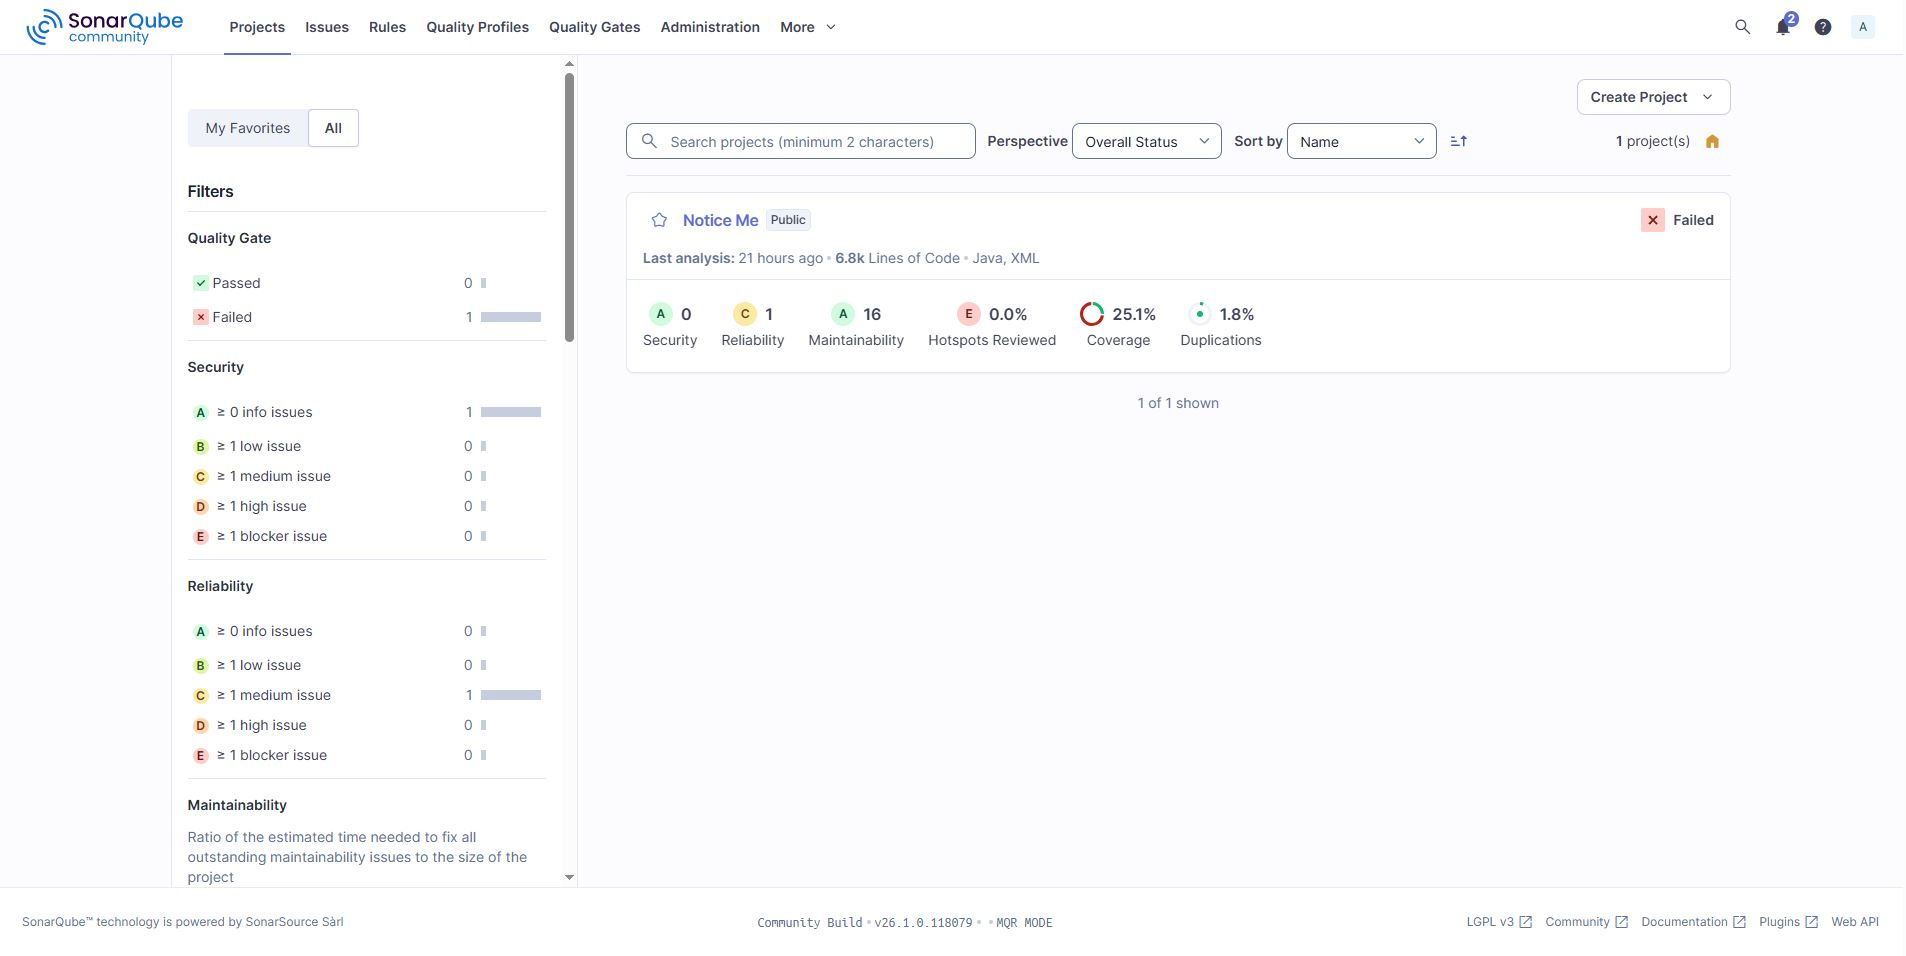
\includegraphics[width=\textwidth]{sonar-main.jpg}
	\caption{Pagina principale del progetto su SonarQube con l'esito del Quality Gate.}
	\label{fig:sonar-quality-gate}
\end{figure}

\begin{figure}[H]
	\centering
	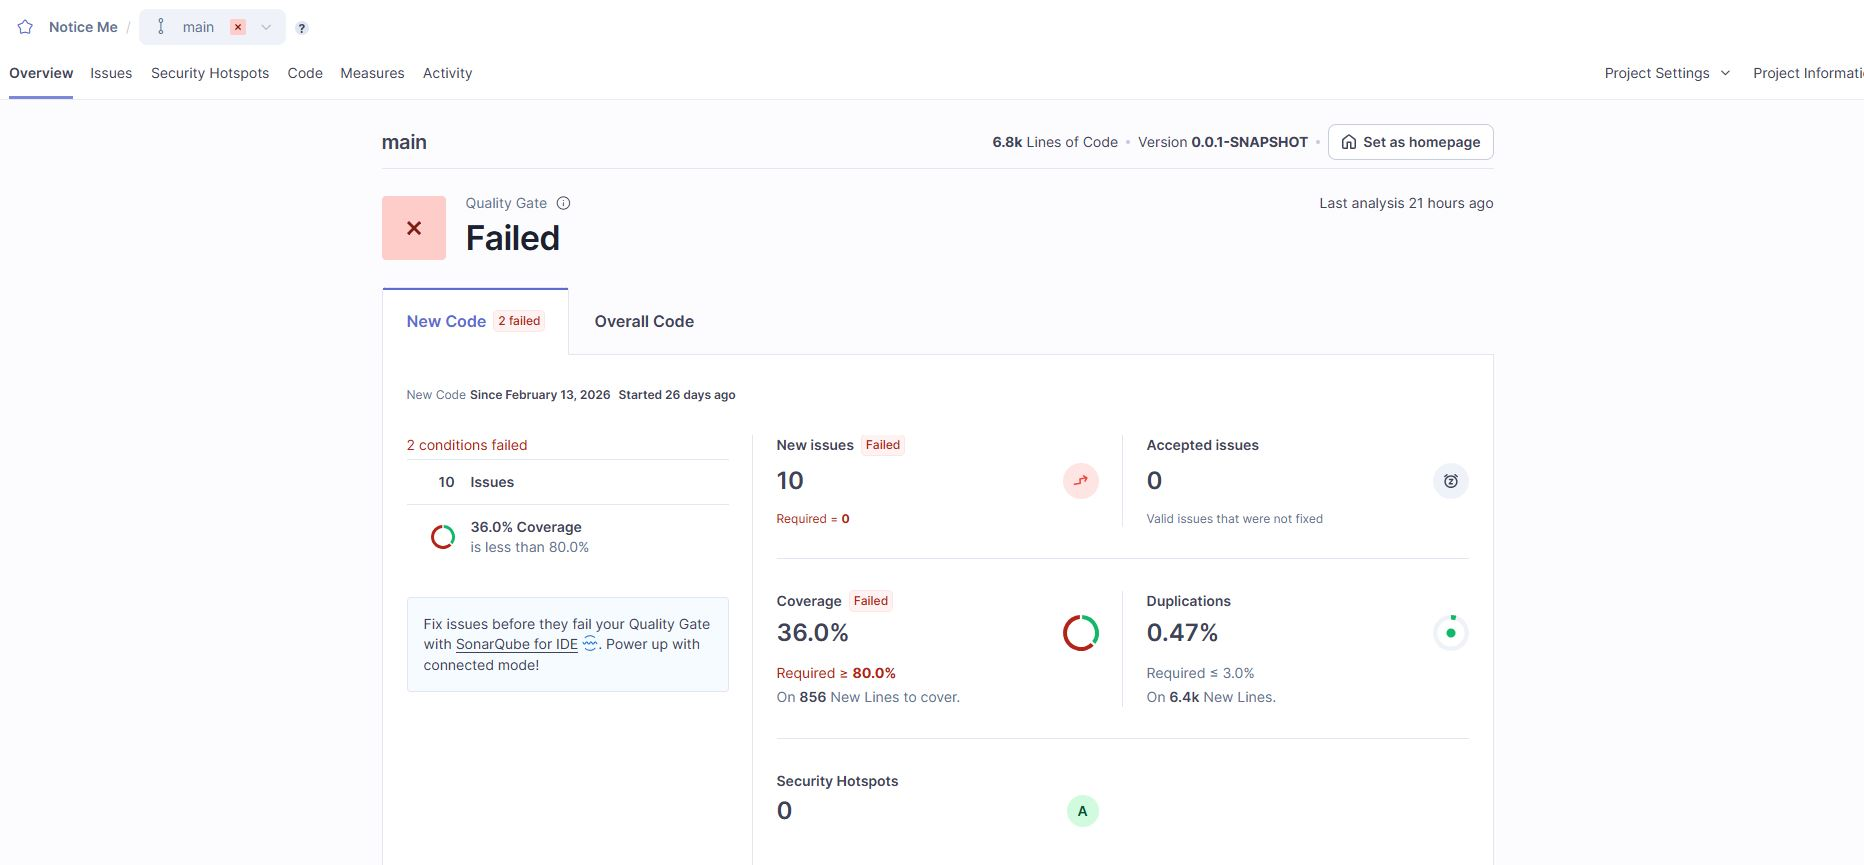
\includegraphics[width=\textwidth]{sonar-overview.jpg}
	\caption{Vista Overview di SonarQube con le principali metriche di qualità del progetto.}
	\label{fig:sonar-overview-img}
\end{figure}

\begin{figure}[H]
	\centering
	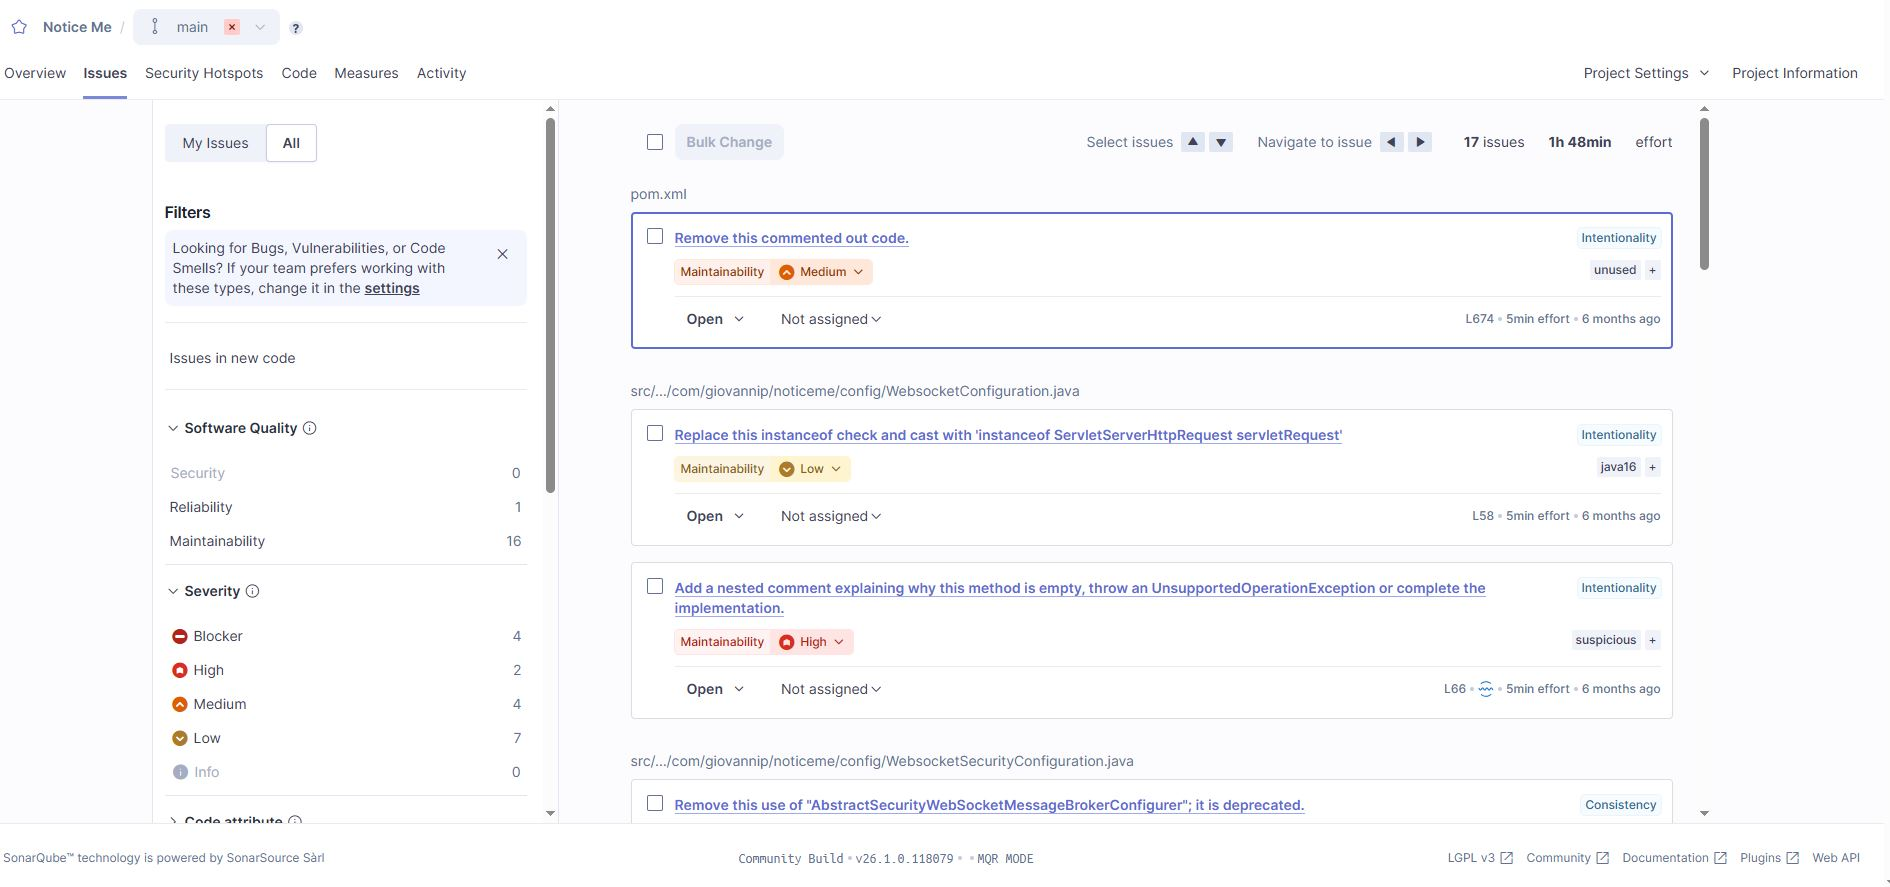
\includegraphics[width=\textwidth]{sonar-issues.jpg}
	\caption{Sezione Issues di SonarQube con i problemi individuati dall'analisi statica del codice.}
	\label{fig:sonar-issues}
\end{figure}

\subsection{Build di rilascio e packaging in produzione}
\label{sub:release}

Sul branch \texttt{main} la pipeline esegue una build di produzione e produce un’immagine Docker tramite \texttt{jib:build} \cite{JibDocs} per costruire l’immagine senza richiedere un Dockerfile esplicito per il backend, pubblicandola su un registry locale.

\Needspace{12\baselineskip}
\captionsetup{type=listing}
\captionof{listing}{Estratto Jenkinsfile: build di rilascio e pubblicazione immagine}
\label{lst:jenkins-release}
\begin{minted}{groovy}
	stage('Release Build') {
		when { branch 'main' }
		steps {
			sh './mvnw -ntp -Pprod clean package -DskipTests'
			sh """
				./mvnw -Pprod jib:build \
				-Djib.to.image=localhost:15000/noticeme:${env.GIT_COMMIT}
			"""
		}
	}
\end{minted}

\subsubsection{Esempio di deploy semplificato}
Una volta pubblicata l’immagine nel registry, il deploy può essere eseguito in modo relativamente semplice sul nodo di destinazione. Il server che ospita l’applicazione scarica l’immagine dal registry e avvia un nuovo container passando la configurazione necessaria, ad esempio il profilo \texttt{prod} e i parametri di connessione al database MySQL. In uno scenario semplificato, il deploy consiste quindi in tre passaggi: recupero dell’immagine, avvio del container e verifica del corretto avvio del servizio.

Un possibile comando di esecuzione è il seguente:

\captionsetup{type=listing}
\captionof{listing}{Esempio semplificato di deploy del container}
\label{lst:docker-run-deploy}
\begin{minted}{bash}
docker pull localhost:15000/noticeme:<tag>

docker run -d \
	--name noticeme-app \
	-p 8080:8080 \
	-e SPRING_PROFILES_ACTIVE=prod \
	-e SPRING_DATASOURCE_URL=jdbc:mysql://mysql:3306/noticeme \
	-e SPRING_DATASOURCE_USERNAME=noticeme \
	-e SPRING_DATASOURCE_PASSWORD=noticeme \
	localhost:15000/noticeme:<tag>
\end{minted}
% !TEX root = ../Thesis.tex

\chapter{Valutazione critica del caso di studio}
\label{cap:evaluation}

Questo capitolo interpreta criticamente i risultati emersi nel caso di studio, con l’obiettivo di rispondere alla domanda di ricerca della tesi: in che misura un framework di generazione full-stack come JHipster supporta concretamente l’adozione di metodologie orientate alla qualità del software, in particolare Test-Driven Development (TDD), Behavior-Driven Development (BDD) e Continuous Integration (CI)?

L’analisi svolta nei capitoli precedenti mostra che JHipster non impone una metodologia di sviluppo specifica, ma fornisce una base architetturale e tecnologica che rende relativamente agevole l’introduzione di pratiche di testing multilivello e di automazione del ciclo di build e verifica.

\section{Valutazione del supporto al Test-Driven Development}
\label{sec:evaluation-tdd}

Dal punto di vista del Test-Driven Development, JHipster offre un contesto favorevole soprattutto in termini di testabilità strutturale. L’architettura generata separa chiaramente dominio, persistenza, service layer, controller REST e frontend, permettendo di individuare precisione i punti in cui introdurre logica applicativa e test mirati. Questa organizzazione rende più semplice la scrittura di test di integrazione e facilita anche il refactoring, poiché ogni livello mantiene responsabilità ben definite.

Un primo elemento positivo è rappresentato dalla suite iniziale di test generata automaticamente dal framework. Tali test, pur non nascendo da un processo TDD in senso stretto, forniscono una rete di sicurezza immediata sulle operazioni CRUD, sulle validazioni di base, sulla serializzazione JSON e sul comportamento degli endpoint REST. In pratica, il progetto dispone fin dall’inizio di un primo insieme di verifiche che riduce il rischio di errori infrastrutturali e semplifica l’evoluzione successiva dell’applicazione. Il TDD non si applica alla nascita del progetto, ma si colloca soprattutto nella sua evoluzione, quando il comportamento standard generato dal framework non è più sufficiente a soddisfare i requisiti del dominio. Nel complesso, si può affermare che JHipster non sia un framework \emph{TDD-first}, ma che fornisca una base fortemente predisposta alla testabilità.

\todo{Inserire qui un dato quantitativo sul numero di test generati automaticamente rispetto a quelli aggiunti manualmente durante il caso di studio.}

\section{Valutazione del supporto al Behavior-Driven Development e E2E}
\label{sec:evaluation-bdd}

Per quanto riguarda il Behavior-Driven Development, il supporto offerto da JHipster è meno diretto rispetto a quello osservato per il testing di integrazione e per la CI. Il framework non genera automaticamente una suite significativa di scenari comportamentali, ma la struttura del progetto e l’integrazione con Spring Boot rendono comunque possibile l’adozione di strumenti come Cucumber senza particolari ostacoli architetturali.

Nel caso di studio, il BDD ha avuto soprattutto un ruolo complementare. Da un lato, ha mostrato la fattibilità dell’integrazione con Cucumber; dall’altro, ha evidenziato che il beneficio di tale approccio dipende fortemente dal contesto organizzativo. In un progetto sviluppato individualmente, infatti, il valore aggiunto del BDD come linguaggio condiviso tende a ridursi.

Una considerazione analoga vale per i test end-to-end con Cypress. Pur non coincidenti con il BDD, essi condividono l’attenzione verso il comportamento osservabile del sistema e consentono di verificare il corretto funzionamento dell’applicazione dal punto di vista dell’utente finale. Nel caso di studio, i test E2E si sono rivelati particolarmente utili dopo la personalizzazione dell’interfaccia relativa alle note, poiché i test generati automaticamente non risultavano più pienamente aderenti al comportamento reale della UI.

Nel complesso, JHipster risulta compatibile con il BDD e con i test end-to-end, ma richiede una scelta metodologica consapevole e un intervento manuale maggiore rispetto ai livelli di test già scaffolded dal framework.

\section{Valutazione del supporto alla Continuous Integration}
\label{sec:evaluation-ci}

L’ambito in cui JHipster mostra il supporto più solido è probabilmente quello della Continuous Integration. Il framework genera infatti un progetto già compatibile con strumenti di build, testing, containerizzazione e packaging moderni, riducendo notevolmente il costo iniziale necessario per costruire un processo di verifica automatizzato.

Nel caso di studio, questa predisposizione ha permesso di realizzare una pipeline Jenkins locale articolata su più livelli di controllo: esecuzione di test unitari e di integrazione, pubblicazione di report JUnit e JaCoCo, generazione di report Cucumber, integrazione di SonarQube per l’analisi statica, esecuzione opzionale di PIT e Gatling, costruzione dell’immagine Docker e pubblicazione in un registry locale. Il risultato è un processo di qualità completo, che va ben oltre la semplice automazione della build.

Il contributo di JHipster risulta particolarmente evidente proprio in questo ambito: il framework non fornisce una pipeline definitiva pronta per ogni scenario, ma mette a disposizione una base tecnica molto favorevole all’automazione, sulla quale è possibile costruire un processo CI coerente, modulare e sostenibile anche in un progetto di dimensioni contenute.

\todo{Inserire qui un riepilogo sintetico dei risultati della pipeline: coverage finale, esito del Quality Gate, mutation score PIT, eventuali report pubblicati e numero totale di stage principali.}

\section{Sintesi critica del sistema di testing}
\label{sec:evaluation-testing-system}

Uno degli aspetti più rilevanti emersi dal caso di studio è la possibilità di costruire, a partire da uno scaffolding generato automaticamente, un sistema di testing stratificato e coerente. I test di integrazione hanno verificato il comportamento delle API REST e della persistenza; i test frontend con Jest hanno coperto la logica lato client; gli scenari Cucumber hanno formalizzato alcuni comportamenti ad alto livello; i test end-to-end con Cypress hanno validato il comportamento complessivo del sistema; infine, mutation testing e analisi statica hanno aggiunto una valutazione qualitativa della robustezza della suite di test e della qualità del codice.

Il valore di questo sistema non risiede soltanto nella quantità di strumenti integrati, ma nella loro complementarità. I livelli di test più rapidi intercettano regressioni frequenti e problemi locali; quelli più costosi vengono invece riservati a scenari funzionali più significativi o a fasi specifiche della pipeline. In questo senso, il caso di studio mostra che JHipster non solo permette l’integrazione di più livelli di test, ma rende anche relativamente naturale il loro inserimento in un processo automatizzato di build e verifica.

\todo{Inserire una tabella o un diagramma riassuntivo dei livelli di test adottati, con indicazione di obiettivo, strumento e fase della pipeline in cui vengono eseguiti.}

Un punto di forza riguarda la predisposizione all’automazione. La compatibilità con Docker, Maven, Jenkins, SonarQube e altri strumenti DevOps rende JHipster particolarmente adatto a essere inserito in pipeline di qualità anche piuttosto articolate. Nel caso di studio, ciò ha consentito di costruire un processo CI locale completo senza dover reingegnerizzare profondamente la struttura del progetto.

\section{Limiti osservati}
\label{sec:evaluation-limits}

Accanto ai vantaggi, il caso di studio ha evidenziato anche alcuni limiti.

Un limite riguarda la qualità semantica dei test generati automaticamente. Sebbene essi siano utili come prima rete di sicurezza, verificano soprattutto aspetti infrastrutturali o CRUD e non coprono in modo automatico i vincoli di business più interessanti. Esiste quindi il rischio di sopravvalutare il livello reale di qualità del progetto se ci si limita ai test scaffolded senza introdurre verifiche di dominio più significative.

Una seconda criticità riguarda il frontend. La generazione automatica dell’interfaccia è molto efficace finché il progetto rimane vicino al modello CRUD standard proposto dal framework. Quando però la UI viene personalizzata in modo sostanziale, come nel caso della gestione delle note del progetto sviluppato, i test jest e E2E generati automaticamente diventano meno aderenti al comportamento effettivo dell’applicazione e devono essere adattati o riscritti.

\section{Limiti dello studio e minacce alla validità}
\label{sec:evaluation-validity}

Le conclusioni tratte nel presente lavoro devono essere interpretate alla luce di alcune limitazioni metodologiche, legate sia alla natura del caso di studio sia agli indicatori utilizzati per valutarne i risultati.

In primo luogo, il progetto sviluppato rappresenta un caso di studio di complessità intermedia. L’applicazione include relazioni tra entità, vincoli di proprietà dei dati, personalizzazioni rispetto allo scaffolding standard e una pipeline di testing e CI relativamente articolata. Tuttavia, non si tratta di un sistema enterprise di larga scala né di un’architettura distribuita su più servizi. Di conseguenza, i risultati osservati non possono essere generalizzati automaticamente a tutti i contesti applicativi.

\todo{Inserire una breve caratterizzazione quantitativa del progetto: numero di entità, classi principali, righe di codice backend/frontend, numero totale di test, numero di commit oppure ampiezza temporale dello sviluppo.}

Un secondo elemento riguarda l’ambiente sperimentale. La pipeline è stata realizzata in un’infrastruttura locale basata su Docker, Jenkins, SonarQube e registry privato. Questa scelta ha il vantaggio della riproducibilità e del controllo completo dell’ambiente, ma potrebbe non riflettere pienamente la complessità organizzativa e operativa di pipeline cloud-based o integrate in ecosistemi aziendali più strutturati.

Dal punto di vista della validità esterna, va inoltre considerato che il caso di studio utilizza una configurazione specifica di JHipster: architettura monolitica, frontend Angular, autenticazione JWT e database SQL. Configurazioni differenti, ad esempio basate su microservizi, gateway o framework frontend alternativi, potrebbero produrre risultati almeno in parte diversi. Anche l’uso di H2 in sviluppo e MySQL in produzione rappresenta un possibile fattore di variabilità.

Dal punto di vista della validità costruttiva, la valutazione si basa su metriche come code coverage, mutation score e indicatori di qualità statica del codice. Sebbene tali metriche forniscano evidenze quantitative importanti, esse non esauriscono il concetto di qualità del software. Una copertura elevata non garantisce automaticamente l’efficacia dei test; un mutation score elevato non misura direttamente la comprensibilità del codice, la qualità del design o la manutenibilità architetturale di lungo periodo. Le metriche utilizzate devono quindi essere lette come indicatori complementari e non come misure esaustive della qualità.

\todo{Inserire una tabella finale con coverage, mutation score, numero totale di test e principali risultati SonarQube.}

Un’ulteriore limitazione è legata al fatto che il progetto è stato sviluppato in modo individuale. Questo semplifica l’analisi e il controllo del caso di studio, ma riduce la possibilità di osservare pienamente alcuni benefici tipici del BDD e della CI in contesti collaborativi, dove la condivisione dei requisiti, la code review e l’automazione del processo assumono un ruolo ancora più rilevante.

Nel complesso, tali limiti non invalidano i risultati ottenuti, ma suggeriscono di interpretarli come evidenze contestualizzate. Il contributo del caso di studio è quindi prevalentemente valutativo ed esplorativo: esso mostra in modo concreto come la generazione automatica del codice possa convivere con pratiche orientate alla qualità, senza pretendere di formulare conclusioni universalmente generalizzabili.
% !TEX root = ../Thesis.tex

\chapter{Conclusioni e sviluppi futuri}
\label{cap:conclusions}

La presente tesi ha analizzato in che misura un framework di generazione full-stack come JHipster possa supportare l’adozione di metodologie orientate alla qualità del software, con particolare riferimento a Test-Driven Development (TDD), Behavior-Driven Development (BDD) e Continuous Integration (CI). L’indagine è stata condotta attraverso un duplice percorso: da un lato l’inquadramento teorico delle metodologie considerate, dall’altro la realizzazione e la valutazione di un caso di studio concreto sviluppato a partire da uno scaffolding generato dal framework.

\section{Sintesi del lavoro svolto}

Nel corso del lavoro è stata progettata e sviluppata un’applicazione di gestione note, caratterizzata da un dominio sufficientemente realistico da consentire l’osservazione di problematiche tipiche dello sviluppo software moderno: relazioni molti-a-molti, vincoli di proprietà dei dati, personalizzazione del comportamento CRUD generato automaticamente e adattamento dell’interfaccia utente rispetto allo scaffolding iniziale.

Su questa base sono stati analizzati diversi livelli di testing e automazione. In particolare, il progetto ha integrato test di integrazione backend, test frontend con Jest, scenari BDD con Cucumber, test end-to-end con Cypress, mutation testing con PIT e analisi statica con SonarQube all’interno di una pipeline CI locale realizzata con Jenkins e Docker.

L’esperienza maturata ha mostrato che JHipster consente di partire rapidamente da una base applicativa coerente e già predisposta alla verifica automatizzata. Allo stesso tempo, il caso di studio ha evidenziato che la qualità finale del sistema non dipende unicamente dal codice generato, ma dalla capacità dello sviluppatore di estendere in modo consapevole lo scaffolding iniziale, introducendo test mirati, vincoli di dominio e un processo di integrazione continua adeguato.

\section{Risposta alla domanda di ricerca}

Alla luce dell’analisi teorica e sperimentale, si può concludere che JHipster supporta in modo concreto pratiche di sviluppo orientate alla qualità, ma con intensità differenti a seconda della metodologia considerata.

Per quanto riguarda il TDD, la struttura architetturale prodotta da JHipster risulta fortemente testabile e rende il TDD particolarmente efficace nella fase evolutiva del progetto, soprattutto quando occorre introdurre regole di business non coperte dallo scaffolding standard.

Per quanto riguarda il BDD e E2E, JHipster non offre un supporto nativo particolarmente forte, ma risulta compatibile con l’integrazione di strumenti come Cucumber e Cypress. Il BDD appare quindi come una pratica applicabile, utile soprattutto nella formalizzazione di comportamenti ad alto livello, ma dipendente da una scelta metodologica esplicita e dal contesto organizzativo in cui il progetto viene sviluppato.

L’ambito in cui JHipster esprime il proprio potenziale in modo più evidente è la Continuous Integration. Il framework facilita infatti la costruzione di pipeline automatizzate, l’integrazione con strumenti di qualità, la containerizzazione e il packaging dell’applicazione, rendendosi particolarmente adatto a contesti di sviluppo orientati all’automazione del processo di build e verifica.

In termini complessivi, la risposta alla domanda di ricerca può essere formulata come segue: JHipster non impone una metodologia specifica, ma costituisce un abilitatore tecnico efficace per l’adozione disciplinata di pratiche orientate alla qualità, con un supporto particolarmente forte alla Continuous Integration, buono alla testabilità e più indiretto al BDD e E2E.

\section{Principali contributi della tesi}

Il principale contributo del lavoro svolto consiste nell’aver mostrato, attraverso un caso di studio concreto, che la generazione automatica del codice non è in contraddizione con l’adozione di pratiche rigorose di testing e automazione. Al contrario, se utilizzata in modo consapevole, essa può ridurre il costo iniziale di avvio del progetto e consentire di concentrare l’attenzione sugli aspetti a maggior valore applicativo, quali la modellazione del dominio, la qualità dei test e la strutturazione del processo di verifica.

Un secondo contributo riguarda la valutazione critica del rapporto tra scaffolding automatico e metodologie test-driven. Il caso di studio ha infatti evidenziato che il codice generato costituisce una buona base iniziale, ma non sostituisce la necessità di progettare esplicitamente i vincoli di dominio, introdurre test significativi e adattare gli strumenti di verifica alle evoluzioni del progetto.

Infine, la tesi mostra che anche in un contesto locale, riproducibile e a costo contenuto è possibile costruire un processo di quality assurance articolato, integrando livelli diversi di test, analisi statica e automazione CI in modo coerente con un progetto generato da JHipster.

\section{Sviluppi futuri}

Il lavoro svolto apre diverse possibili direzioni di approfondimento.

Un primo sviluppo naturale consiste nell’estendere l’analisi a configurazioni architetturali differenti di JHipster, in particolare al paradigma a microservizi. Questo permetterebbe di osservare come TDD, BDD e CI si comportino in presenza di maggiore complessità distribuita, comunicazione tra servizi e pipeline multi-componente.

Un secondo possibile sviluppo riguarda il rafforzamento della valutazione empirica. Sarebbe utile condurre un confronto sistematico con altri framework o generatori full-stack, oppure con un’applicazione sviluppata manualmente, al fine di valutare con maggiore precisione l’impatto della generazione automatica sul testing e sull’automazione del processo di sviluppo.

Dal punto di vista applicativo, il caso di studio potrebbe essere esteso introducendo funzionalità ulteriori, come la condivisione delle note tra utenti, la gestione di ruoli differenziati, la collaborazione multiutente o meccanismi di notifica. Tali estensioni renderebbero il dominio più ricco e offrirebbero ulteriori occasioni per analizzare vincoli di business complessi e scenari di test avanzati.

Infine, sul piano infrastrutturale, potrebbe risultare interessante portare la pipeline in un contesto cloud o semi-distribuito, integrando registry remoti, ambienti di staging, deployment automatizzato e monitoraggio post-rilascio.

In conclusione, il caso di studio conferma che la generazione automatica del software, se accompagnata da consapevolezza metodologica e controllo della qualità, non rappresenta un’alternativa alle buone pratiche di ingegneria del software, ma un possibile acceleratore della loro adozione.


%--------------------------------------------------------------
% Bibliography
%--------------------------------------------------------------
\bibliographystyle{plain} 
\bibliography{Bibliography} % Entries are in the Bibliography.bib file

%--------------------------------------------------------------
\end{document}
%--------------------------------------------------------------
